\section{Analýza}
V tejto kapitole sa venujeme rozboru dostupných platforiem pre e-learning matematiky. 
Cieľom je identifikovať platformy, porovnať ich funkcie a odhaliť medzery, ktoré naša webová aplikácia môže vyplniť. 
Na trhu existuje široká škála platforiem pre e-learning rôznych matematických tém, 
z ktorých každá ponúka rôzne riešenia, funkcie a zameriava sa na odlišné cieľové skupiny.

\subsection{Brilliant.org}
Online vzdelávacia platforma Brilliant.org poskytuje interaktívne kurzy v rôznych oblastiach vedy, či už matematickej alebo počítačovej.
 Kurzy sú prispôsobené rôznym vedomostným úrovniam, od začiatočníkov až po pokročilých a platforma ich ponúka viac ako 60.
 Brilliant.org je výborným nástrojom na rozvíjanie kritického myslenia a logických schopností, pretože je navrhnutá tak, aby podporovala aktívne učenie problémov a interaktívnych výziev.

 Hlavnými výhodami platformy sú interaktívne lekcie, ktoré sú navrhnuté tak, aby boli pútavé a aby vyžadovali aktívnu účasť študentov.
  Na to slúžia denné výzvy rôznych tém – tie udržujú študentov motivovaných, neustále zapojených do procesu učenia a zvyšujú efektivitu ich štúdia.
   Platforma tiež umožňuje flexibilné a  samostatné štúdium a je teda vhodná aj pre individuálne potreby.
  Jej nevýhodou je však skutočnosť, že je platená a dostupná len v anglickom jazyku, čo sa niektorým študentom môže javiť ako prekážka.\cite{brilliant}
\subsection{Khan Academy}
Khan Academy je platforma poskytujúca bezplatné videokurzy a interaktívne cvičenia z rovnakých oblastí ako Brilliant.org (matematickej a počítačovej vedy).
 Disponuje širokou škálou obsahu a zdrojmi k daným témam, ktoré sú prehľadné a dobre štruktúrované. Je dostupná pre rôzne úrovne znalostí – je vhodná pre študentov základných, stredných, ale aj vysokých škôl.
 Ponúka možnosť sledovania pokroku, získavania bodov a odznakov za splnené kapitoly a tým motivuje študentov k učeniu prostredníctvom gamifikácie.

 Nevýhodou je opäť dostupnosť iba v anglickom jazyku a používateľské rozhranie, ktoré sa niektorým používateľom môže javiť ako neprehľadné, najmä ak sa na platforme nachádzajú prvýkrát.\cite{khanacademy}
\subsection{Vieme matiku}
Vieme matiku je najpopulárnejší slovenský portál na e-learning matematiky.
 Je určený pre žiakov základných a stredných škôl a jeho veľkou výhodou je teda oproti vyššie spomenutým platformám, jeho dostupnosť pre slovenských žiakov.
 Kurzy a cvičenia, ktoré portál poskytuje sa venujú širokému okruhu tém a ponúkajú taktiež hravé prvky, zvyšujúce motiváciu žiakov – napr. grafické a zvukové efekty.
 K ďalším prednostiam portálu patrí možnosť rôznych foriem precvičovania, grafické znázornenie úloh, možnosť sledovania pokroku a tiež jednoduché použitie a prehľadné rozhranie.
 Nevýhodou je, že platforma neponúka zdroje pre samostatné štúdium, nápovedy a nie je dostupná pre študentov mimo Slovenska, keďže je podporovaná iba v slovenskom jazyku.
 Zároveň, v prípade, že by sme chceli naplno využiť všetky jej funkcie, by bolo potrebné si zakúpiť licenciu.\cite{viemeto}
\subsection{Zhodnotenie}
Analýza súčasných vzdelávacích platforiem nás priviedla k zisteniu, že na trhu chýbajú lokalizované a cenovo dostupné e-learningové riešenia pre stredoškolských a vysokoškolských študentov, ktoré by účinne kombinovali gamifikáciu, interaktivitu a prehľadné rozhranie. 
Vyššie spomenuté platformy, ako Brilliant.org a Khan Academy síce disponujú kvalitnými vzdelávacími materiálmi, no ich dostupnosť je limitovaná anglickým jazykom a v prípade Brilliant.org aj plateným modelom.
Nevýhodou slovenského portálu Vieme matiku je zase fakt, že nezohľadňuje pokročilé potreby samostatného štúdia a je obmedzená na úzky okruh používateľov.
Analyzované platformy ukázali širokú škálu prístupov k vzdelávaniu. 
Mnohé z nich sa zameriavajú na riešenie komplexných úloh alebo tradičné formy vzdelávania, no často nekladú dôraz na intuitívne osvojovanie matematických konceptov a podporu samostatného učenia.
Tieto poznatky nám umožnili identifikovať nedostatky súčasných vzdelávacích platforiem a formulovať jasné požiadavky na vývoj novej aplikácie, ktorá by ponúkala lokalizovaný obsah, interaktívne učenie a dostupnosť pre rôzne cieľové skupiny.

\begin{table}[htbp]
\caption{Vzdelávacie platformy}
\label{vzdelavaciePlatformy}
\begin{tabularx}{\textwidth}{|X|X|X|X|}
\hline
\textbf{Platforma} & \textbf{Funkcie} & \textbf{Cieľová skupina} & \textbf{Cena} \\ \hline
Khan Academy & Videokurzy, cvičenia & Všetky úrovne & Bezplatná \\ \hline
Brilliant.org & Gamifikované kurzy & Stredné a Vysoké školy & Platená \\ \hline
Vieme Matiku & Online kurzy matematiky & Základné a Stredné školy & Čiastočne bezplatná \\ \hline
\end{tabularx}
\end{table}

\section{Použité technológie a knižnice}
V tejto kapitole sa podrobne venujeme technológiám a knižniciam, ktoré plánujeme
použiť na vývoj webovej aplikácie pre e-learning matematickej štatistiky a
pravdepodobnosti. Výber technológií je založený na princípoch flexibility,
kompatibility, bezpečnosti a aktívnej komunity vývojárov.


\subsection{Frontend}
Frontend je časť softvérového vývoja, ktorá sa zaoberá tým, čo používateľ vidí a s čím interaguje pri práci s aplikáciou alebo webovou stránkou. 
Ide o viditeľnú vrstvu aplikácie, ktorá zahŕňa všetky prvky používateľského rozhrania (\acrshort{ui}) a je priamo zodpovedná za používateľskú skúsenosť (\acrshort{ux}).

V kontexte nášho webového vývoja predstavuje frontend technológie a nástroje používané na tvorbu webových stránok, ktoré sú dostupné a vykresľované v internetových prehliadačoch. 
Zahŕňa návrh, implementáciu a optimalizáciu používateľského rozhrania tak, aby bolo esteticky príťažlivé, funkčné a dostupné na rôznych zariadeniach a platformách.
\subsubsection{HTML}
\acrfull{html} je značkovací jazyk používaný na tvorbu a štruktúrovanie obsahu webových stránok.
Je schopný definovať rôzne prvky, ako sú nadpisy, odseky, obrázky či odkazy, čím určuje základnú kostru a vzhľad webovej stránky.
Napriek častým mylným predstavám, HTML nie je programovací jazyk, keďže neumožňuje vytvárať podmienené logické operácie alebo funkcie.
Jeho hlavnou úlohou je prezentácia a organizácia obsahu pre webové prehliadače. 
\cite{HTML}

\subsubsection{CSS}
\acrfull{css} je štýlovací jazyk používaný na definovanie vzhľadu a formátovania webových stránok. 
Slúži na oddelenie vizuálnej prezentácie od štruktúry obsahu definovanej v \acrshort{html}, čím zjednodušuje údržbu a aktualizáciu dizajnu.
Pomocou \acrshort{css} je možné nastaviť rôzne vizuálne vlastnosti, ako sú farby, písma, veľkosti, rozloženie prvkov a ďalšie aspekty dizajnu.
 Podporuje taktiež tvorbu responzívnych dizajnov, ktoré sa prispôsobujú rôznym zariadeniam a veľkostiam obrazoviek. 
 Moderné techniky, ako flexbox a grid, umožňujú presné rozmiestnenie a zarovnanie prvkov na stránke, čo je užitočné pri tvorbe komplexných rozložení.\cite{css}

\subsubsection{SCSS}
\acrfull{scss} je rozšírenie jazyka \acrshort{css}, ktoré pridáva pokročilé funkcie pre efektívnejšie štýlovanie webových stránok. 
\acrshort{scss} umožňuje používať premenné, vnáranie selektorov, mixiny, funkcie a operácie, a tak uľahčuje zjednodušuje správu a údržbu štýlov.
 Vďaka svojim vlastnostiam podporuje modulárny prístup k tvorbe štýlov, čím zlepšuje čitateľnosť kódu a urýchľuje vývoj.

 \acrshort{scss} používa štandardnú \acrshort{css} syntax s doplnením nových funkcií, čo zabezpečuje spätnú kompatibilitu.
 Kód napísaný v \acrshort{scss} sa následne kompiluje do klasického \acrshort{css}, ktoré podporujú všetky moderné prehliadače. 
Tento proces zvyšuje flexibilitu vývoja a poskytuje možnosť tvorby komplexných štýlových štruktúr.\cite{scss}
\subsubsection{JavaScript}
JavaScript je interpretovaný programovací jazyk, ktorý slúzi na dynamickú interakciu s používateľom a zmeny obsahu webových stránok bez nutnosti ich opätovného načítania.

Podporuje objektovo orientované programovanie s triedami, objektmi a metódami, čo umožňuje tvorbu komplexných aplikácií. Vďaka svojej dynamickej povahe dokáže meniť obsah a štruktúru stránky počas jej behu.

Medzi jeho funkcie patrí funkcionálne programovanie, kde sú funkcie považované za prvotriedne objekty, a programovanie riadené udalosťami, ktoré umožňuje reagovať na interakcie používateľa, napríklad na kliknutia.

Je multiplatformový a podporuje rôzne zariadenia, ako sú počítače, smartfóny a tablety. Populárne knižnice a rámce ako jQuery, React, Angular a Vue výrazne uľahčujú vývoj aplikácií.

Medzi jeho vlastnosti patrí manipulácia s \acrfull{dom}, spracovanie udalostí, manipulácia s dátami a podpora asynchrónnych volaní na server pomocou techniky \acrfull{ajax}.
 Tieto vlastnosti z neho robia základný nástroj na tvorbu moderných webových aplikácií.\cite{JavaScript}
 \subsubsection{AJAX}
 AJAX (Asynchronous JavaScript and XML) je technológia, cez ktorú môžu webové aplikácie načítavať a odosielať dáta na pozadí bez nutnosti obnoviť celú stránku.
  Funguje na kombinácii známych technológií – HTML, CSS, JavaScript a XMLHttpRequest (alebo moderného fetch) – a výrazne zlepšuje interaktivitu a používateľskú skúsenosť. 
 AJAX sa využíva napríklad v ankete bez reloadu, našeptávačoch alebo moderných single-page aplikáciách.\cite{ajax}
\subsubsection{jQuery}
jQuery je open-source knižnica napísaná v JavaScripte, ktorá uľahčuje prácu s HTML dokumentom, manipuláciu s DOM, prácu s udalosťami, animáciami a technológiou AJAX.
 Bola vytvorená v roku 2006 s cieľom zjednodušiť vývoj v čase, keď neexistovala jednotná podpora v prehliadačoch.
  Aj napriek tomu, že je dnes považovaná za technicky zastaranú a dátovo náročnú, stále sa používa na mnohých weboch vďaka svojej jednoduchosti a veľkému množstvu dostupných pluginov.\cite{jquery}


 \subsubsection{TypeScript}
TypeScript je programovací jazyk vyvinutý spoločnosťou Microsoft, ktorý rozširuje možnosti JavaScriptu pridaním statického typovania a pokročilých objektovo orientovaných prvkov.
 Tým pomáha vývojárom identifikovať chyby už počas vývoja, čo zvyšuje spoľahlivosť a udržiavateľnosť kódu.
  TypeScript je nadmnožinou JavaScriptu, čo znamená, že všetok platný kód v JavaScripte je kompatibilný s TypeScriptom.
   Po napísaní sa kód v TypeScripte transpiluje do štandardného JavaScriptu, ktorý je podporovaný vo všetkých moderných prehliadačoch. 
   Tento prístup umožňuje využívať výhody moderných programovacích techník pri zachovaní širokej kompatibility a flexibility, ktorú JavaScript ponúka.\cite{TypeScript} 
\subsubsection{MathJax}
MathJax je open-source\footnote{Open-source je softvér, ktorého zdrojový kód je voľne dostupný, môže byť používaný, upravovaný a distribuovaný kýmkoľvek.} JavaScriptový engine určený na zobrazovanie matematických notácii, ako sú LaTeX, MathML a AsciiMath, v moderných webových prehliadačoch.
Je navrhnutý tak, aby konsolidoval pokroky vo webových technológiách do jednotnej platformy pre matematiku na webe, podporujúc hlavné prehliadače a operačné systémy, vrátane mobilných zariadení.
Používatelia nemusia inštalovať žiadne doplnky ani softvér; stačí, aby autor stránky zahrnul MathJax a matematický obsah do webovej stránky, a MathJax sa o zvyšok postará.\cite{MathJax}


  \subsubsection{MathQuill}
  MathQuill je open-source webový editor matematických výrazov navrhnutý tak, aby bol schopný jednoducho a esteticky zadávať matematiku priamo v prehliadači. 
  Umožňuje používateľom zadávať a zobrazovať matematické výrazy v známej vizuálnej forme pomocou syntaxe podobnej LaTeXu.

Je obľúbený v edukatívnych a interaktívnych webových aplikáciách, pretože poskytuje dynamické pole, v ktorom možno editovať matematické vzorce s okamžitým vizuálnym výstupom. 
MathQuill podporuje rôzne režimy – ako zobrazenie statických výrazov, interaktívne polia pre vstup používateľa alebo čítanie/zápis LaTeX kódu.\cite{mathquill}
\subsubsection{ApexCharts}
ApexCharts je open-source JavaScriptová knižnica určená na vizualizáciu dát v podobe interaktívnych grafov.
 Poskytuje širokú škálu grafických typov a umožňuje ich jednoduchú integráciu do webových aplikácií s podporou populárnych frameworkov ako React, Angular či Vue. 
Vďaka svojej flexibilite, responzívnosti a podpore dynamických dát sa často využíva pri tvorbe analytických nástrojov a interaktívnych dashboardov.\cite{apexcharts}

\subsection{Backend}
Backend predstavuje časť softvérovej aplikácie, ktorá nie je priamo prístupná používateľom; ide o serverovú stranu v klient-server architektúre.
 Zodpovedá za hlavnú funkcionalitu aplikácie, vrátane spracovania webových požiadaviek, manipulácie s dátami a ich ukladania v databázach. Backend spolupracuje s frontendom, ktorý tvorí prezentačnú vrstvu aplikácie, s cieľom zabezpečiť komplexnú používateľskú skúsenosť. 
 Dáta generované na backende sú odosielané na frontend, kde sú prezentované používateľovi.
  Hoci sú často backend a frontend vyvíjané oddelenými tímami, hranica medzi nimi môže byť nejasná, čo vedie k prístupu známemu ako full-stack\footnote{Full-stack vývoj je proces, kde vývojár pracuje na frontende aj backende, teda na používateľskom rozhraní aj serverovej logike.} development, kde programátori pracujú na oboch stranách aplikácie.
   V minulosti backend pozostával prevažne z jednoduchých serverových skriptov, avšak s rozvojom webových technológií sa využívajú pokročilé frameworky umožňujúce dynamickú generáciu obsahu.
 Efektívny backendový kód je kľúčový pre optimalizáciu výkonu aplikácie, minimalizáciu zaťaženia servera a databázy, a zabezpečenie rýchlej odozvy pre používateľov. \cite{backend} 
 \subsubsection{API}
 \acrfull{api} je rozhranie, ktoré slúži na komunikáciu jednej aplikácie s inou aplikáciou alebo systémom.
 Umožňuje vývojárom využívať už existujúce funkcionality bez toho, aby ich museli znova vytvárať, čím urýchľuje a simplifikuje tak vývoj softvéru.
  \acrshort{api} definuje spôsob výmeny dát medzi klientom a serverom. \cite{api}
 \subsubsection{REST}
 \acrshort{rest} \acrshort{api} \acrfull{rest} \acrfull{api} je typ webového \acrshort{api}, vďaka ktorému môžu medzi sebou aplikácie komunikovať pomocou štandardných \acrshort{http} protokolov. 
 REST API využíva jednoduché operácie ako čítanie, zápis, úprava a mazanie dát prostredníctvom \acrshort{url} adries a HTTP metód.

Jeho výhodou je jednoduchá štruktúra, škálovateľnosť a nezávislosť medzi klientom a serverom – klient nemusí poznať vnútornú logiku servera a server nemusí vedieť nič o klientskom rozhraní.
 REST API je široko používané pri vývoji moderných webových a mobilných aplikácií, pretože zabezpečuje flexibilnú a efektívnu výmenu dát.\cite{rest}
\subsubsection{CORS}
CORS (Cross-Origin Resource Sharing) predstavuje mechanizmus, ktorý umožňuje realizáciu HTTP požiadaviek medzi rôznymi doménami (tzv. cross-origin požiadavky).
 Ide o spôsob, akým môžu prehliadače bezpečne vykonávať požiadavky na zdroje umiestnené na iných serveroch, než odkiaľ pochádza pôvodná webová stránka. 
 V minulosti takýmto požiadavkam bránila politika rovnakého pôvodu (same-origin policy), ktorá obmedzovala skripty bežiace v prehliadači výhradne na komunikáciu so serverom tej istej domény.

Mechanizmus CORS funguje tak, že server explicitne definuje, kto môže vytvárať požiadavky na jeho \acrshort{api}
, aké typy požiadaviek sú povolené a aké HTTP metódy sú podporované.
 Toto sa realizuje prostredníctvom špeciálnych HTTP hlavičiek, ktoré napomáhajú prehliadaču určiť, či konkrétna požiadavka medzi rôznymi doménami môže byť bezpečne vykonaná.\cite{CORS}
\subsubsection{Node.js}
Node.js je runtime\footnote{Runtime prostredie je prostredie poskytujúce aplikácii všetky potrebné zdroje, knižnice a služby, ktoré sú potrebné na jej spustenie a beh.}
prostredie umožňujúce použitie JavaScriptu na strane servera, pričom využíva flexibilitu a jednoduchosť tohto programovacieho jazyka.
 Výhodou JavaScriptu sú jeho pokročilé koncepty ako „first-class functions“ (funkcie prvej triedy) a closures, ktoré dokážu vytvoriť efektívne webové aplikácie. 
 Hoci JavaScript býva kritizovaný za nespoľahlivosť, táto kritika vyplýva predovšetkým zo zvláštností \acrshort{dom}-u v prehliadačoch, nie zo samotného jazyka.
 \subsection{Databázové systémy}
 Databázový systém je softvérové riešenie, ktoré slúži na uchovávanie, správu a vyhľadávanie dát. 
 Umožňuje vytvárať databázy, ktoré obsahujú štruktúrované dáta usporiadané v tabuľkách, a poskytuje nástroje na ich úpravu, triedenie, filtrovanie a prezentáciu.
 
 Databáza samotná je organizovaný súbor údajov, často rozdelený do tabuliek, ktoré spolu súvisia a medzi ktorými môžu byť definované vzťahy. 
 Cieľom databázového systému je zabezpečiť integritu, konzistenciu a dostupnosť dát, pričom používateľ môže s dátami pracovať pomocou formulárov, dotazov či zostáv.\cite{databazovesystemy}
 
 \subsubsection{SQL}
 \acrfull{sql} je jazyk navrhnutý na prácu s dátami v relačných databázach, ktorý umožňuje ich optimalizované ukladanie, organizáciu a získavanie.
 V \acrshort{sql} sa údaje ukladajú do tabuliek, ktoré fungujú ako dvojrozmerné štruktúry zložené z riadkov a stĺpcov. 
 Každá tabuľka predstavuje určitý typ objektu (napr. zákazníci, produkty) a každý riadok v tabuľke predstavuje jeden záznam s konkrétnymi údajmi.
 
 Pomocou dotazov (queries) je možné z databázy získať presne tie údaje, ktoré používateľ potrebuje – napríklad filtrovať podľa podmienok, zoskupovať dáta alebo ich spájať z viacerých tabuliek.
 Dotazy sú základom práce s \acrshort{sql} a vedia analyzovať, transformovať a prezentovať uložené informácie v požadovanej forme.\cite{sql}
 
 \subsubsection{PostgreSQL}
 PostgreSQL je pokročilý open-source objektovo-relačný databázový systém (\acrshort{ordbms}), ktorý kombinuje tradičné vlastnosti relačných databáz so schopnosťou pracovať s objektovo orientovanými prvkami. 
 To znamená, že okrem práce s tabuľkami a vzťahmi (typických pre \acrfull{rdbms}) podporuje aj vlastné dátové typy, dedičnosť, či ukladanie komplexných štruktúr, ako sú napríklad JSON či geografické dáta.
 
 Ako \acrshort{ordbms}, PostgreSQL umožňuje definovať vlastné funkcie, procedúry a typy, vďaka čomu ponúka vysokú mieru prispôsobiteľnosti pre náročné aplikácie. 
 Je navrhnutý s dôrazom na integritu dát, rozšíriteľnosť a štandardy \acrshort{sql}, a preto je široko používaný v podnikových riešeniach, výskumných systémoch aj moderných webových aplikáciách.\cite{postgre}
 \subsubsection{DBDiagram}
 dbdiagram.io je bezplatný online nástroj, ktorý vývojárom a dátovým analytikom slúži na jednoduché vytváranie diagramov databázových štruktúr pomocou nekomplikovaného textového zápisu.
 Jeho hlavnou výhodou je schopnosť rýchlo a efektívne navrhovať a vizualizovať databázové schémy, a tak uľahčiť plánovanie a komunikáciu v tímoch.
 Používatelia môžu definovať tabuľky, stĺpce a vzťahy medzi nimi v jednoduchom jazyku, pričom nástroj automaticky generuje zodpovedajúci diagram.
 Okrem toho dbdiagram.io podporuje import a export SQL skriptov, čo zabezpečuje integráciu s existujúcimi databázami a uľahčuje migráciu alebo dokumentáciu databázových štruktúr.
 Vďaka týmto funkciám je dbdiagram.io obľúbeným nástrojom pre rýchly návrh databáz a spoluprácu na databázových projektoch.
 \subsection{Framework}
 Framework je softvérová platforma poskytujúca vývojárom preddefinovanú štruktúru a nástroje, ktoré urýchľujú a zjednodušujú proces vývoja aplikácií.
 Existujú rôzne typy frameworkov podľa oblasti použitia, napríklad webové, desktopové či mobilné.
 Používanie frameworkov prináša výhody ako rýchlejší vývoj, lepšiu kvalitu kódu a štandardizáciu práce vývojárov. \cite{framework}
 \subsubsection{Frontendové frameworky}
 Frontend framework je špecializovaný typ frameworku určený na vývoj používateľských rozhraní webových aplikácií.
 Na rozdiel od všeobecných frameworkov, ktoré môžu pokrývať celý vývojový cyklus aplikácie, frontend framework sa sústreďuje výhradne na klientskú časť – teda na to, čo používateľ vidí a s čím interaguje v prehliadači.
 Poskytuje nástroje a štruktúru na organizáciu komponentov, správu stavu aplikácie a manipuláciu s \acrshort{dom}-om, optimalizuje a na základe tohto disponuje možnosťou tvorby dynamických, responzívnych a udržiavateľných rozhraní.
 \subsubsection{Rozdiel medzi CSS a JavaScript (JS) frameworkami}
 \begin{itemize}
  \item CSS frameworky (napr. Bootstrap, Tailwind CSS, Materialize) sú zamerané na vizuálnu stránku webu – poskytujú hotové štýly, rozloženia, komponenty (tlačidlá, formuláre, mriežky), ktoré zjednodušujú tvorbu konzistentného a estetického dizajnu. Ide predovšetkým o „vzhľad“ aplikácie.
  \item JS frameworky (napr. React, Angular, Vue.js) naopak poskytujú funkčnú logiku a štruktúru aplikácie. 
  Umožňujú pracovať s dátami, dynamicky meniť obsah stránky bez opätovného načítania (tzv. \acrshort{spa}), pracovať s API a definovať správanie komponentov.\cite{feframework}
\end{itemize}
\subsubsection{Angular}
Angular je open-source framework vyvinutý spoločnosťou Google, určený na tvorbu dynamických a responzívnych webových aplikácií.
Pomáha vývojárom vytvárať aplikácie s bohatou funkcionalitou prostredníctvom komponentovo orientovanej architektúry, ktorá podporuje opätovné použitie kódu a optimalizuje údržbu aplikácií.
Angular využíva TypeScript, nadmnožinu JavaScriptu, ktorá pridáva statické typovanie a ďalšie funkcie zlepšujúce vývojový proces. 
Medzi kľúčové vlastnosti Angularu patrí obojsmerná väzba dát, ktorá synchronizuje model a zobrazenie, a modulárny systém, ktorý rozdeľuje aplikácie na menšie, ľahko spravovateľné časti.
Angular tiež obsahuje nástroje na správu formulárov, komunikáciu so serverom a smerovanie, vďaka čomu dokážu vývojári vytvárať komplexné aplikácie s minimálnym úsilím. \cite{angular}

\subsubsection{RxJs}
\acrshort{rxjs} \acrfull{rxjs} je knižnica určená na reaktívne programovanie, ktorá zabezpečuje efektívne spracovanie asynchrónnych a udalostne založených dátových tokov pomocou tzv. observables. 
Tieto observables predstavujú prúdy dát (napr. kliknutia, HTTP odpovede), ktoré môžu byť pozorované a spracovávané rôznymi operátormi ako map, filter či reduce.

RxJS umožňuje prehľadnejšie a konzistentnejšie riadiť komplexné interakcie v aplikáciách, najmä tam, kde dochádza k častým zmenám stavu alebo udalostiam v čase.
Využíva sa najmä v moderných frontend frameworkoch, ako je Angular, kde zjednodušuje prácu s dátami a udalosťami.\cite{rxjs}
\subsubsection{Backendové frameworky}
Back-end framework je softvérový nástroj, ktorý uľahčuje vývoj serverovej časti webovej aplikácie. 
Poskytuje štruktúru, komponenty a funkcie potrebné na spracovanie požiadaviek, prácu s databázou, autentifikáciu a ďalšie serverové operácie. 
Cieľom back-end frameworku je zefektívniť vývoj, zabezpečiť konzistentnosť kódu a podporiť štandardizované riešenia. 
Rôzne frameworky (napr. Django, Spring, Laravel, Ruby on Rails, Express) sa líšia podľa náročnosti projektu, škálovateľnosti, dokumentácie a vhodnosti pre začiatočníkov či veľké podnikové aplikácie.\cite{backendframework}

\subsubsection{Express.js}
Express je JavaScriptový framework fungujúci ako ľahká nadstavba nad Node.js, ktorý zjednodušuje tvorbu webových aplikácií a \acrshort{api}.
Zatiaľ čo Node.js poskytuje základné prostredie pre spúšťanie JavaScriptu na serveri, Express pridáva štruktúru a pomáha vývojárom vyhnúť sa opakovanému a zdĺhavému písaniu nízkoúrovňového kódu. 
Express je teda nástroj, ktorý optimalizuje a zrýchľuje vývoj tým, že poskytuje vyššiu úroveň abstrakcie oproti základným funkciám dostupným v čistom Node.js.

Jeho minimalistická architektúra ponúka veľkú mieru flexibility – vývojári nie sú nútení dodržiavať presne stanovenú štruktúru projektu, no zároveň majú k dispozícii nástroje na efektívne spracovanie HTTP požiadaviek, tvorbu routovacích pravidiel a využívanie middleware vrstiev. 
Express umožňuje jednoduché vytváranie \acrshort{rest}ful \acrshort{api} a dynamických webových aplikácií.
Pre svoju jednoduchosť, rozsiahlu dokumentáciu a silnú komunitu patrí medzi najpopulárnejšie riešenia pre serverovú časť aplikácií postavených na JavaScripte.\cite{express}\cite{backendframework}
\subsection{UI a UX}
Používateľské rozhranie predstavuje vizuálnu časť digitálneho produktu, s ktorou používateľ priamo interaguje. 
Zahŕňa prvky ako tlačidlá, ikony, typografiu a farebné schémy. 
Cieľom UI dizajnu je vytvoriť esteticky príjemné a funkčné prostredie, ktoré uľahčuje používateľovi navigáciu a interakciu s produktom.

Používateľský zážitok sa zameriava na celkovú skúsenosť používateľa pri interakcii s produktom alebo službou. 
Ide o to, ako intuitívne a rýchlo dokáže používateľ dosiahnuť svoje ciele. 
UX dizajn zahŕňa analýzu potrieb používateľov, návrh informačnej architektúry, prototypovanie a testovanie, s cieľom zabezpečiť, aby bol produkt nielen funkčný, ale aj príjemný na používanie.

Hoci sú UI a UX dve rozličné disciplíny, úzko spolupracujú s cieľom vytvoriť digitálne produkty, ktoré sú však taktiež použivateľsky prívetivé.\cite{uiux}
\subsubsection{Figma}
Figma je cloudová platforma slúžiaca na vytvorenie návrhu a prototypovanie používateľských rozhraní pre webové a mobilné aplikácie. 
Umožňuje tímovú spoluprácu v reálnom čase prostredníctvom webového prehliadača alebo desktopovej aplikácie. Podporuje vektorové ilustrácie, interaktívne prototypy a dizajnové systémy.
 Všetky projekty sú uložené v cloude, a tento fakt spôsobuje, že je k nim lepší prístup a dajú sa jednoduchšie zdieľať. \cite{figma}
 \subsubsection{Material UI}
 Angular Material UI je oficiálna knižnica komponentov pre Angular, ktorá implementuje dizajnové princípy Material Design od spoločnosti Google. 
 Poskytuje predpripravené a prispôsobiteľné komponenty, ako sú tlačidlá, formuláre, tabuľky či navigačné panely, a tak dokážu vývojári rýchlo vytvárať moderné, responzívne a esteticky príjemné používateľské rozhrania.
  Angular Material UI podporuje integráciu s Angular frameworkom a zabezpečuje konzistentný dizajn a vysokú úroveň použiteľnosti v rámci aplikácií. \cite{materialUI}

\subsection{Gamifikácia v e-learningu}
Gamifikácia v e-learningu zahŕňa integráciu herných prvkov, ako sú body, odznaky, rebríčky a úrovne, do vzdelávacích online prostredí s cieľom zvýšiť motiváciu a angažovanosť študentov.
 Podľa príspevku v zborníku z medzinárodnej vedeckej konferencie "Vzdělávání dospělých 2021" \cite{gamifikacia} je gamifikácia efektívnym nástrojom na podporu aktívneho učenia, pretože využíva prirodzenú ľudskú tendenciu k hre a súťaživosti.
  Implementácia herných mechanizmov v e-learningových kurzoch môže viesť k zlepšeniu zapojenia študentov, zvýšeniu ich motivácie a následne k lepším vzdelávacím výsledkom.

\subsection{Server}
Server je centrálny počítač v sieti, ktorý poskytuje služby a zdroje iným zariadeniam – tzv. klientom. 
Dajú sa na ňom uchovávať a sprístupňovať dáta, spúšťať aplikácie, spracovávať požiadavky používateľov alebo poskytovať webové stránky či e-mailové služby.
 Môže ísť o fyzický počítač alebo virtuálny stroj a jeho konkrétna funkcia závisí od typu – existuje napríklad súborový, databázový, aplikačný alebo webový server. 
 Správne nastavený server je základom spoľahlivej a bezpečnej IT infraštruktúry.\cite{server}
\subsubsection{NGINX}
Nginx je výkonný a spoľahlivý webový a reverzný proxy server, ktorý je navrhnutý na rýchle spracovanie veľkého množstva súčasných pripojení pri minimálnom využití systémových zdrojov. 
Najčastejšie sa používa na poskytovanie statického obsahu, ako sú HTML, CSS, JavaScript alebo obrázky, a zároveň ako sprostredkovateľ medzi klientom a backend aplikáciou, čím preposiela požiadavky na servery bežiace napríklad v Node.js alebo PHP. 
Nginx dokáže tiež rozdeľovať záťaž medzi viaceré servery, a tak zabezpečiť vyššiu dostupnosť a škálovateľnosť aplikácií, a môže slúžiť ako cache server pre rýchlejšie doručovanie často používaného obsahu.
 Vďaka svojej asynchrónnej architektúre a podpore moderných protokolov, ako sú \acrshort{http}/3 a \acrshort{tls}, je ideálnym riešením pre hosting moderných webových aplikácií s vysokými nárokmi na výkon.\cite{nginx}
\subsubsection{Docker}
Docker je open-source platforma, ktorá umožňuje vývoj, distribúciu a správu aplikácií pomocou tzv. kontajnerov. 
Kontajner je ľahké a izolované prostredie, ktoré obsahuje všetko potrebné na beh aplikácie – vrátane kódu, knižníc, runtime prostredia a nastavení.

Vďaka tomu môže aplikácia bežať rovnakým spôsobom na rôznych miestach, napríklad na vývojárskom počítači, v testovacom prostredí aj na produkčnom serveri. 
Docker využíva virtualizáciu na úrovni operačného systému, a vďaka tomuto dokáže spúšťať viacero kontajnerov naraz s nízkymi nárkomi na systémové prostriedky.\cite{docker}
\subsection{GIT}
Git je distribuovaný systém slúžiaci na správu verzií, ktorým sa dajú sledovať a zaznamenávať zmeny v súboroch počas vývoja softvéru.
 Umožňuje viacerým vývojárom pracovať súčasne na tom istom projekte, pričom každá kópia projektu obsahuje úplnú históriu zmien. 
 Git je známy svojou rýchlosťou, flexibilitou a podporou nelineárnych pracovných tokov. 
Je open-source, bezplatný a vďaka svojim vlastnostiam sa stal štandardom v oblasti verzionovania kódu.\cite{git}

\section{Návrh webovej aplikácie}
Naša webová aplikácia je koncipovaná ako systém s trojvrstvovou architektúrou, ktorá pozostáva z prezentačnej, logickej a dátovej vrstvy. 
Prezentačnú vrstvu (frontend) sme implementovali pomocou frameworku Angular, zatiaľ čo logickú vrstvu (backend) sme vytvorili pomocou platformy Express. 
Fakt, že sme obidve časti navrhnli ako samostatné a na sebe nezávislé aplikácie, nám v procese vytvárania umožnil väčšiu flexibilitu nielen v oblasti samotného vývoja, ale aj testovania či nasadzovania aplikácie na server.
Dátovú vrstvu tvorí databázový systém PostgreSQL, ktorý zaisťuje ukladanie a efektívne spracovanie dát celej aplikácie.

Ako sme už spomenuli v predchádzajúcich kapitolách, backendová časť je zodpovedná za spracovanie údajov, manipuláciu s databázou, \acrshort{ldap} autentifikáciu používateľov a spracovanie požiadaviek zo strany klienta. Ide o akúsi integračnú vrstvu medzi používateľským rozhraním a databázou, ktorá zabezpečuje bezpečný a efektívny prenos údajov. 

Backend sme implementovali pomocou frameworku Express.js, postavenom na Node.js. Dôvodom bola nielen jeho funkcia jednoducho vytvárať \acrshort{rest} \acrshort{api} rozhrania, ale aj dispozícia mnohých ďalších výhod, akými sú jednoduchosť, flexibilita, rozsiahla komunita a množstvo dostupných middleware modulov, čo výrazne urýchľuje vývoj serverovej logiky.

Express.js je zároveň ideálne riešenie pre aplikácie typu \acrshort{spa}, akú predstavuje aj náš frontend vytvorený v Angulari. V tomto architektonickom modeli plní Express úlohu backendovej vrstvy poskytujúcej \acrshort{api} endpointy, prostredníctvom ktorých frontend získava dynamicky obsah a dáta. Táto kombinácia zaisťuje rýchlu a plynulú interakciu používateľa s aplikáciou bez potreby neustáleho obnovovania stránky, čím sa zvyšuje používateľský komfort a celkový výkon systému.

Na efektívne riadenie oprávnení a zabezpečenie rôznych úrovní prístupu k funkcionalitám aplikácie slúži \acrshort{ldap} autentifikácia. Tá overuje identitu používateľov a priraďuje im prístupové práva na základe ich roly, ktorými sú v našej aplikácii študent a administrátor (učiteľ). 

Frontend sme navrhli ako \acrfull{spa} s použitím frameworku Angular. Ten sme vybrali pre jeho výbornú škálovateľnosťou a komponentový prístup, ktorý umožňuje vytvárať zapuzdrené (encapsulované) komponenty. Vďaka tomuto sa kód lepšie organizuje a je viac čitateľný  a lepšie sa preto pracuje na jeho údržbe a opätovnom použití.

Komunikácia medzi frontendom a backendom je sprostredkovaná prostredníctvom tzv. servisných tried (Services), ktoré Angular poskytuje ako jednu zo svojich kľúčových funkcionalít. Tieto služby slúžia na získavanie údajov zo servera, validáciu používateľských vstupov, uchovávanie stavu aplikácie, ako aj na centrálne spracovanie logiky a dát. Každá Angular služba je singleton\footnote{Návrhový vzor, ktorý zabezpečuje, že z určitej triedy existuje v aplikácii práve jedna inštancia, ktorá je globálne dostupná.} objekt a zdieľa dáta a funkcionality naprieč celou aplikáciou, vďaka čomu sa signifikantne zvyšuje modularita systému a podporuje sa znovupoužiteľnosť kódu.

Pri asynchrónnej komunikácii a práci s údajmi sme v Angulari využili mechanizmus Observables, ktorý je súčasťou knižnice \acrshort{rxjs}. Tento mechanizmus dokáže efektívne pracovať s dátovými tokmi, ako sú napríklad \acrshort{http} požiadavky alebo používateľské vstupy, a poskytuje pokročilé možnosti týkajúce sa reaktívneho spracovania dát, zrušenia požiadaviek, spájania viacerých streamov alebo transformácie údajov. Vďaka tejto reaktívnej paradigme dokáže aplikácia flexibilne reagovať na zmeny v dátach a zvyšuje sa jej interaktivita, výkon a stabilita.


\subsection{Špecifikácia}
Primárnym cieľom našej webovej aplikácie je poskytnúť efektívnu a modernú platformu pre študentov, ktorí si chcú prehĺbiť svoje znalosti z matematiky, špeciálne z oblasti teórie pravdepodobnosti.
 V reakcii na obmedzenia a nedostatky súčasných vzdelávacích systémov a aplikácií je naša platforma navrhnutá tak, aby nebola len nástrojom na tvorbu a vyhodnocovanie testov, ale zároveň poskytovala interaktívne študijné materiály a vizualizácie, ktoré zlepšujú pochopenie teoretických konceptov.

Aplikácia kladie dôraz na rozdelenia pravdepodobnosti, pričom podporuje diskrétne rozdelenia ako rovnomerné, binomické, hypergeometrické, poissonovo a geometrické rozdelenie.
 Každé z rozdelení je v aplikácii reprezentované interaktívnymi vizualizáciami a príkladmi, čo študentom umožňuje lepšie porozumieť danej problematike.

Systém zároveň rozlišuje dve hlavné role používateľov – rolu \textit{študenta} a rolu \textit{administrátora (učiteľa)}. Každá z týchto rolí disponuje špecifickými funkcionalitami, ktoré sú prístupné iba na základe autentifikácie používateľa.
 Študentom aplikácia umožňuje prístup k študijným materiálom, generovanie testov a sledovanie svojho pokroku.
  Administrátori majú k dispozícii rozšírené možnosti správy obsahu, vrátane tvorby testov, ako aj monitorovania aktivít a pokroku jednotlivých študentov.

  Pre systematické znázornenie interakcií použivateľov so systémom, sú vytvorené diagramy prípadov použitia zvlášť pre rolu študenta (obrázok č. ~\ref{studentdiagram}) a administrátora (obrázok č. ~\ref{admindiagram}), ktoré súčasťou ďalších kapitol tejto práce.

\subsection{Funkcionálne požiadavky}
Funkcionálne požiadavky sú špecifikácie, ktoré definujú, čo by systém mal robiť a aké funkcie by mal poskytovať používateľom.
 Tieto požiadavky sa zameriavajú na konkrétne správanie systému, interakcie s používateľmi a spracovanie údajov. 
 V našej aplikácii sme identifikovali nasledujúce funkcionálne požiadavky pre študentov a administrátorov:
 \subsubsection{Pre študentov}
 \begin{itemize}
   \item Prihlásenie do systému pomocou \acrshort{ldap} autentifikácie.
   \item Prehliadanie študijných materiálov z oblasti pravdepodobnosti a štatistiky.
   \item Generovanie testov podľa vybraných tém.
   \item Riešenie úloh v rámci testovej sady s možnosťou využitia nápoved.
   \item Zobrazenie výsledkov testov vrátane získaného počtu bodov a použitých nápoved.
   \item Sledovanie vlastného pokroku a úspešnosti pri riešení úloh.
   \item Export testových úloh a výsledkov vo formáte vhodnom na uloženie alebo tlač.
 \end{itemize}
 
\subsubsection{Pre administrátorov (učiteľov)}
\begin{itemize}
  \item Prihlásenie do systému pomocou \acrshort{ldap} autentifikácie ako učiteľ.
\item Zobrazovanie výsledkov všetkých študentov.
\item Prístup k všeobecným štatistikám a analýzam výkonnosti.
\item Pridávanie nových testoých úloh.
\item Správa existujúcich testových úloh vrátane ich úpravy a mazania.
\item Zobrazovanie histórie testov a pokroku jednotlivých študentov.
  \end{itemize}

\subsection{Nefunkcionálne požiadavky}
Nefunkcionálne požiadavky sú špecifikácie, ktoré sa zameriavajú na vlastnosti a kvalitu systému, ako sú výkon, bezpečnosť, použiteľnosť a údržba.
 Tieto požiadavky sa netýkajú konkrétnych funkcií, ale skôr toho, ako by mal systém fungovať a aké vlastnosti by mal mať. 
 V našej aplikácii sme identifikovali nasledujúce nefunkcionálne požiadavky:
 \begin{itemize} 
    \item Jednoduchosť a prehľadnosť používateľského rozhrania – rozhranie musí byť intuitívne, prispôsobené aj menej technicky zdatným používateľom. 
    \item Spoľahlivé a overené študijné materiály – obsah aplikácie je čerpaný z dôveryhodných odborných zdrojov.
    \item Rýchla odozva pri generovaní testov a spracovaní výsledkov – činnosti musia byť vykonané v čo najkratšom čase bez zbytočného čakania.
    \item Podpora rôznych zariadení – aplikácia musí byť plne funkčná na počítačoch, tabletoch aj mobilných zariadeniach. 
    \item Modulárnosť a rozšíriteľnosť systému – systém je navrhnutý tak, aby bolo možné v budúcnosti pridávať nové moduly, úlohy či témy bez nutnosti zásahu do existujúceho jadra aplikácie. 
  \end{itemize}


 \subsection{Diagramy prípadov použitia}
\subsubsection{Diagramy prípadov použitia pre študenta}
\begin{figure}[H]
  \centering
  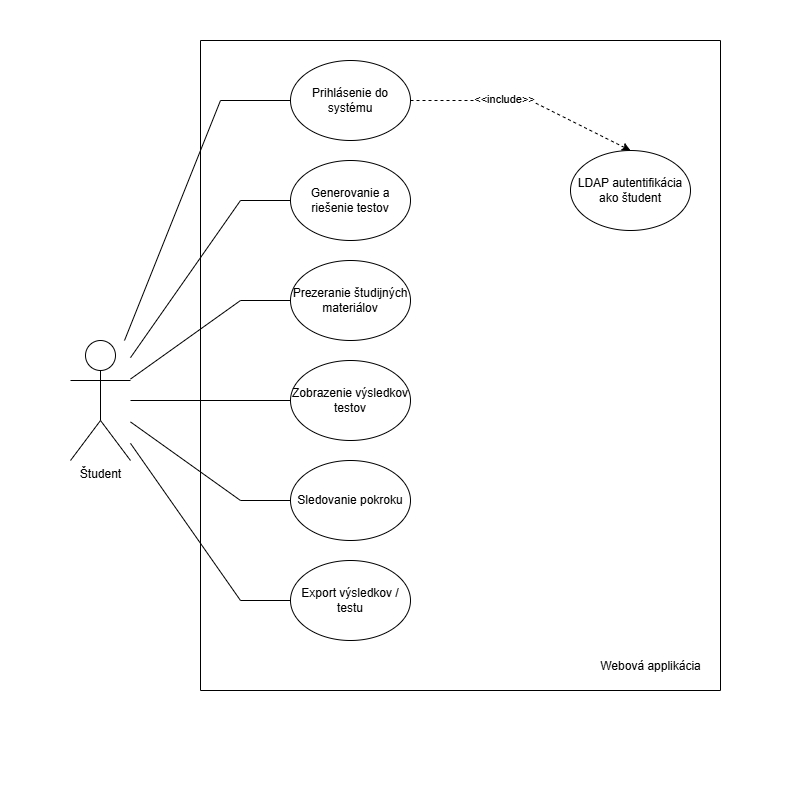
\includegraphics[width=16cm]{img/diagram_student.png}
  \caption{Diagram prípadov použitia pre študenta.}
  \label{studentdiagram}
\end{figure}



\subsubsection{Diagramy prípadov použitia pre administrátora}
\begin{figure}[H]
  \centering
  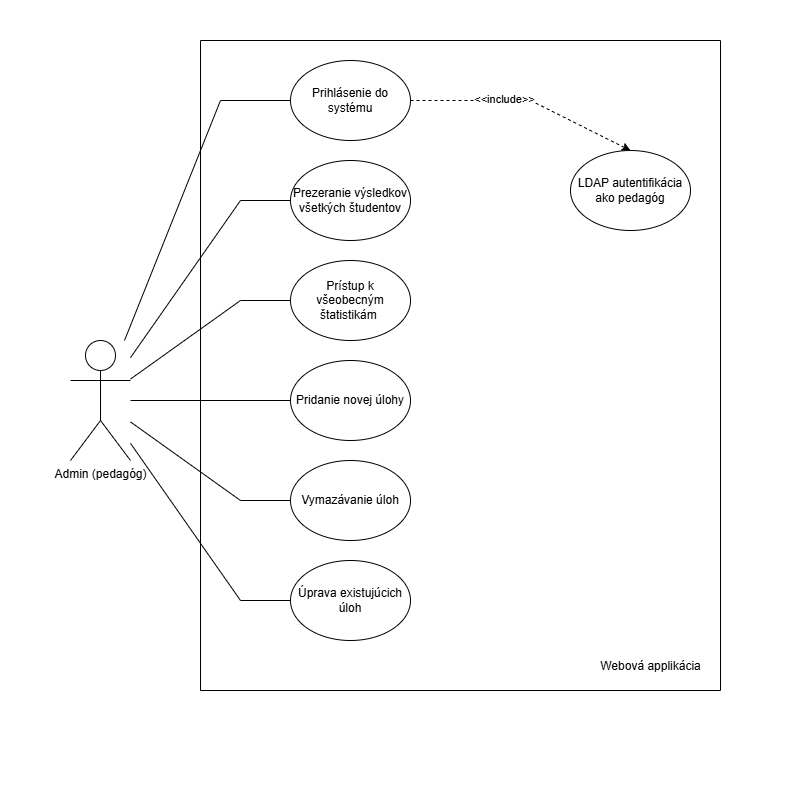
\includegraphics[width=16cm]{img/diagram_admin.png}
  \caption{Diagram prípadov použitia pre administrátora.}
  \label{admindiagram}
\end{figure}



 \subsection{Databáza}
 Databázovým systémom našej webovej aplikácie je PostgreSQL, ktorý sme si zvolili pre jeho flexibilnú prácu s dátami. 
 Využívame najmä podporu pre JSONB, vďaka ktorej vieme efektívne ukladať a vyhľadávať polostruktúrované dáta, ako sú odpovede či nápovedy.

Ďalšou výhodou je podpora poľových typov (ARRAY), ktoré zjednodušujú štruktúru databázy tým, že umožňujú uchovávať viacero hodnôt v jednom stĺpci. 
PostgreSQL nám tak poskytuje výkonné a praktické riešenie pre prácu s komplexnými údajmi.

Okrem uvedených výhod PostgreSQL veľmi dobre spolupracuje s kontajnerizačnou platformou \textbf{Docker}.
Prostredníctvom Docker kontajnerov môžeme jednoducho spustiť databázu s vopred definovanou štruktúrou a údajmi.
Docker taktiež dokáže automatizovať tento proces pomocou bash skriptu, ktorý načíta inicializačné SQL skripty pri spustení kontajnera.
Vďaka tomu je databáza okamžite pripravená na používanie v potrebnej konfigurácii ihneď po spustení kontajnera.

Na obrázku č~\ref{dbtableobr}. je zobrazený logický ER diagram (Entity-Relationship Diagram) databázového modelu našej aplikácie.
 Tento diagram zobrazuje vzťahy medzi jednotlivými entitami a znázorňuje, ako sú údaje v databáze navzájom prepojené.
\begin{figure}[htbp]
  \centering
  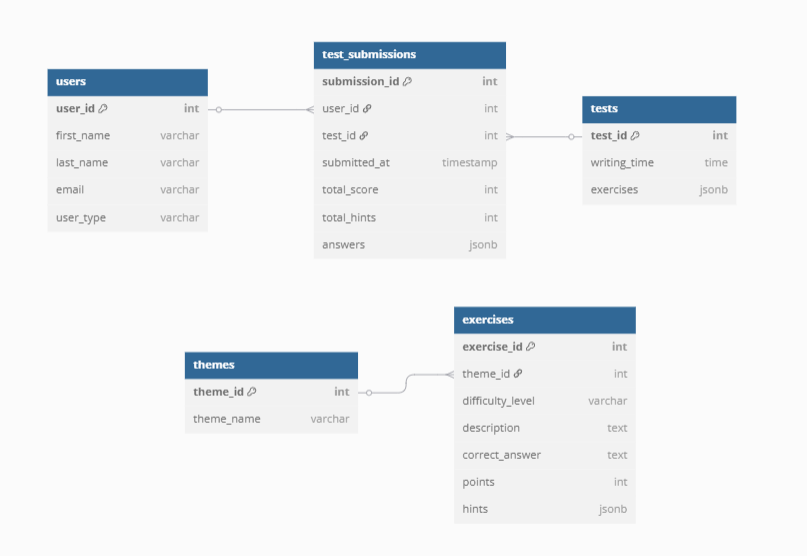
\includegraphics[width=12cm]{img/dbtablefinal.png}
  \caption{Logický ER diagram (Entity-Relationship Diagram) databázového modelu.}
  \label{dbtableobr}
\end{figure} 


Databáza sa skladá z nasledovných tabuliek:
\begin{itemize}
  \item \textit{users} – uchováva informácie o prihlásených používateľoch. 
  Keďže autentifikáciu realizujeme prostredníctvom akademického LDAP systému, neukladáme žiadne citlivé dáta, ktoré by neboli dostupné priamo z \acrshort{ldap}. 
  Okrem základných údajov rozlišujeme aj typ používateľa (študent alebo administrátor/učiteľ), ktorý taktiež získavame z \acrshort{ldap} a ktorý ovplyvňuje rozsah oprávnení v aplikácii.
  \item \textit{themes} - obsahuje zoznam matematických tém, primárne z oblasti matematickej štatistiky, ktoré slúžia na kategorizáciu úloh.
  \item \textit{exercises} - uchováva údaje o jednotlivých úlohách, ako sú zadanie, úroveň obtiažnosti, počet bodov, správna odpoveď a dostupné nápovedy. 
  Každá úloha je priradená k jednej tematickej oblasti (theme\_id).
  \item \textit{tests} - reprezentuje sadu úloh, ktorá sa skladá z kombinácie úloh z databázy a automaticky generovaných úloh. Zároveň obsahuje aj časový limit na vypracovanie testu.
  \item \textit{test\_submissions} -  zaznamenáva konkrétne podania testov jednotlivými používateľmi.
   Obsahuje informácie o tom, kto test riešil, akú testovú sadu dostal, kedy test odovzdal, aké odpovede zadal, koľko bodov získal a koľko nápoved použil.
\end{itemize}

Polia \textit{answers} a \textit{hints} sú uložené vo formáte JSONB, čo umožňuje flexibilne uchovávať komplexné štruktúry dát, ako napríklad zoznam odpovedí alebo počty použitých nápoved ku konkrétnym úlohám.
 Príklad zápisu JSON dát v tomto stĺpci je znázornený na obrázku č.~\ref{dbjsonb}.

 \begin{figure}[h!]
  \centering
  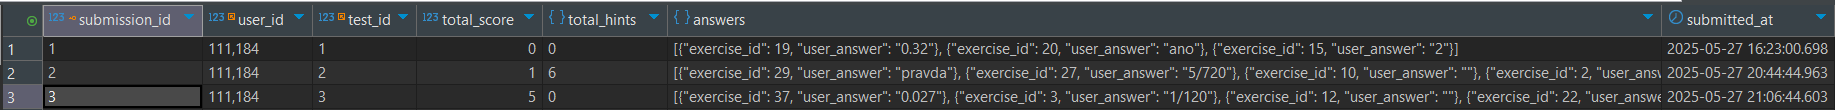
\includegraphics[width=\textwidth]{img/dbjsonb.png}
  \caption{Príklad zápisu JSON dát v stĺpci \textit{answers}.}
  \label{dbjsonb}
 \end{figure}

 Každé zadanie úlohy (description) je uložené ako reťazec vo formáte LaTeX, ktorého prednosťou je pohodlný zápis matematických vzorcov a výrazov. Tento spôsob zápisu je výhodný najmä pre potreby zobrazovania úloh vo webovom rozhraní pomocou renderovacích nástrojov ako je napríklad MathJax, ktoré dokážu LaTeX premeniť na kvalitne vykreslené rovnice.

Príklad zápisu jednej úlohy s použitím LaTeX zápisu je znázornený na obrázku č.~\ref{latexpriklad}.

\begin{figure}[H]
  \centering
  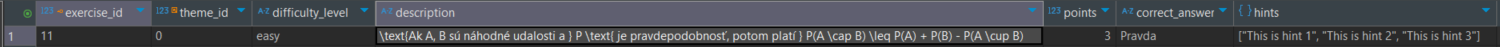
\includegraphics[width=\textwidth]{img/latex_example.png}
  \caption{Ukážka LaTeX zápisu zadania úlohy v databáze}
  \label{latexpriklad}
\end{figure}


\subsection{Použivateľské rozhranie}

Používateľské rozhranie aplikácie bolo navrhnuté s dôrazom na prehľadnosť, jednoduchosť a intuitívnu navigáciu, čím sme chceli docieliť zníženie kognitívnej záťaže používateľa a zvýšiť celkovú používateľskú skúsenosť (UX). Cieľom návrhu bolo zabezpečiť, aby sa aj používateľ s minimálnymi digitálnymi zručnosťami dokázal v prostredí jednoducho orientovať a efektívne pracovať so všetkými funkciami aplikácie.

Základná štruktúra dizajnu bola vytvorená v nástroji Figma, ktorý poskytol vizuálny návrh používateľského rozhrania ešte pred samotnou implementáciou. Rozhranie je koncipované ako hlavné menu s veľkými, vizuálne výraznými blokmi, ktoré reprezentujú jednotlivé kľúčové funkcie aplikácie:
\begin{itemize} 
  \item Písanie testu 
  \item Zobrazenie napísaných testov 
  \item Export testov a výsledkov 
  \item Prístup k študijným materiálom 
\end{itemize}

Ako môžeme vidieť na obrázku č.~\ref{homescreen}, ide o hlavnú obrazovku aplikácie, ktorá slúži ako východiskový bod pre všetky hlavné činnosti používateľa.

\begin{figure}[H]
  \centering
  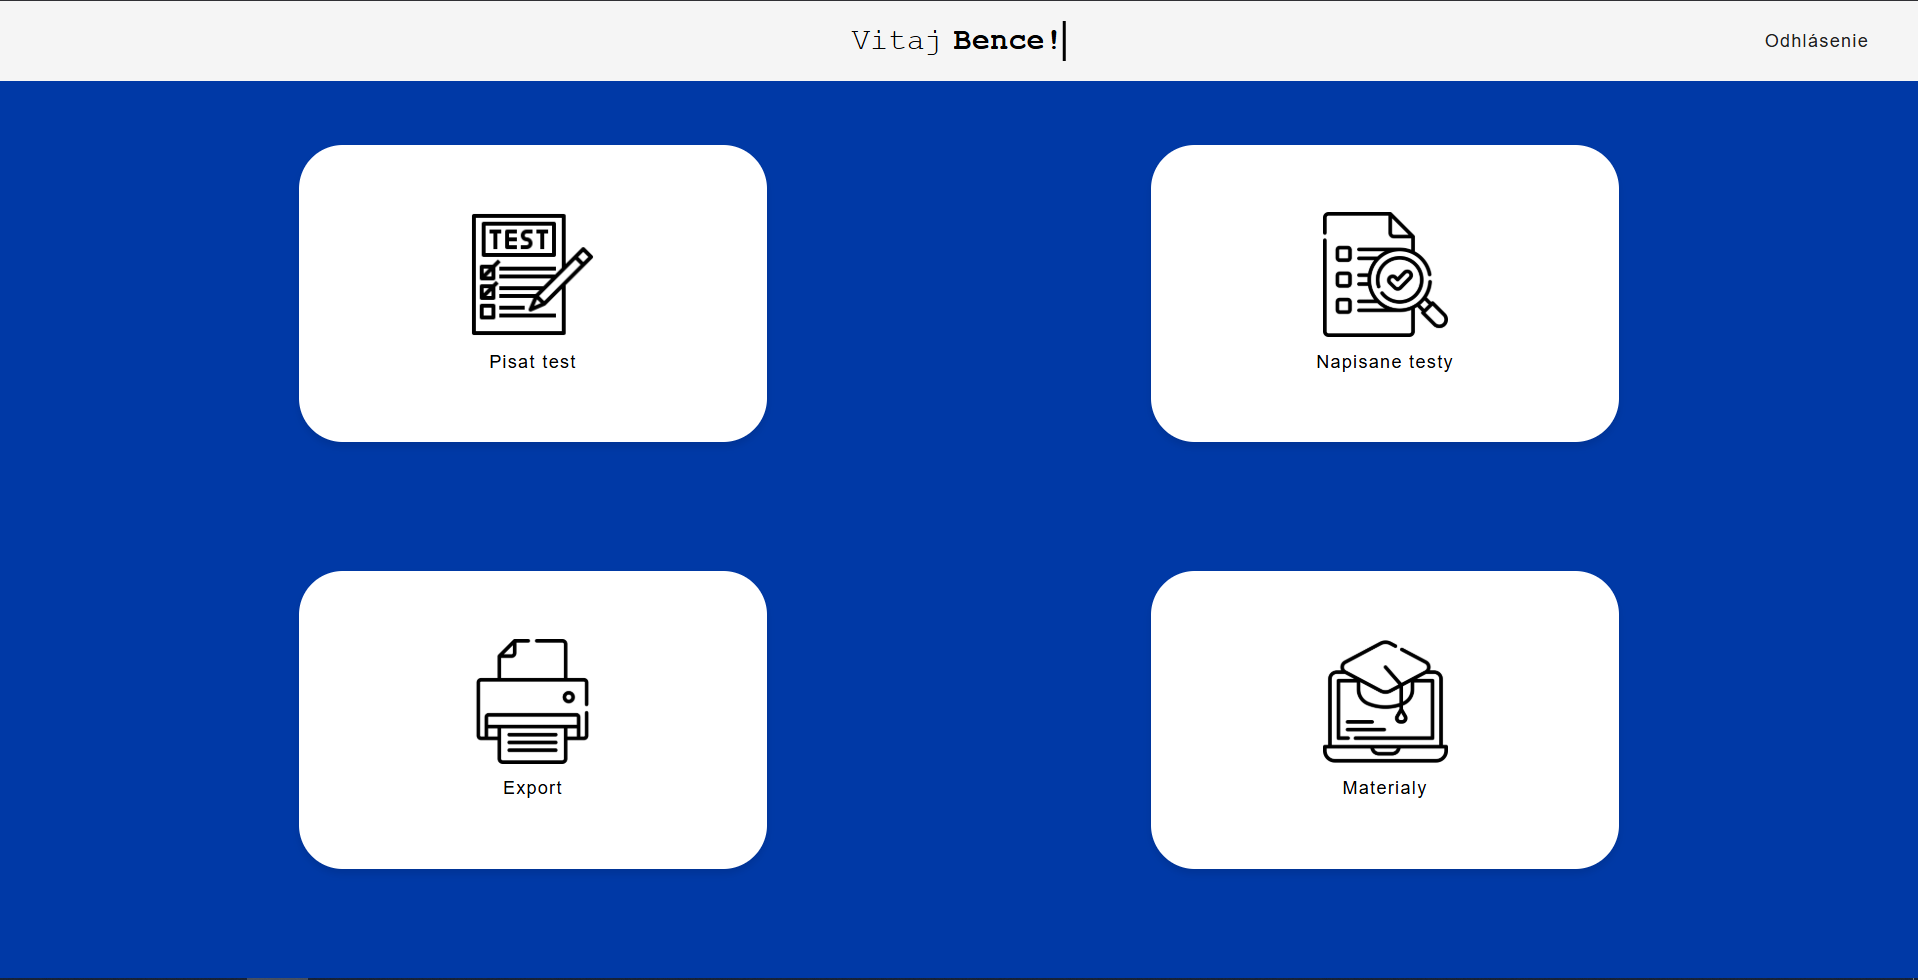
\includegraphics[width=16cm]{img/homepage.png}
  \caption{Hlavná obrazovka aplikácie.}
  \label{homescreen}
\end{figure} 

Navigácia v aplikácii je zabezpečená pomocou horného navigačného panela, ktorý obsahuje možnosť návratu na hlavnú obrazovku a tlačidlo pre odhlásenie zo systému. Tento prvok je dostupný na všetkých podstránkach aplikácie, čím sa zabezpečuje jednotný a konzistentný spôsob navigácie naprieč celým systémom.

Na obrázku č.~\ref{figmavizual} je zobrazený výrez z konceptuálneho návrhu podstránky \textit{Písať test}, ktorý bol súčasťou úvodného vizuálneho návrhu. 
V porovnaní s finálnou implementáciou prešli niektoré prvky úpravami zameranými na lepšiu prehľadnosť, responzívnosť a použiteľnosť používateľského rozhrania.

\begin{figure}[H]
  \centering
  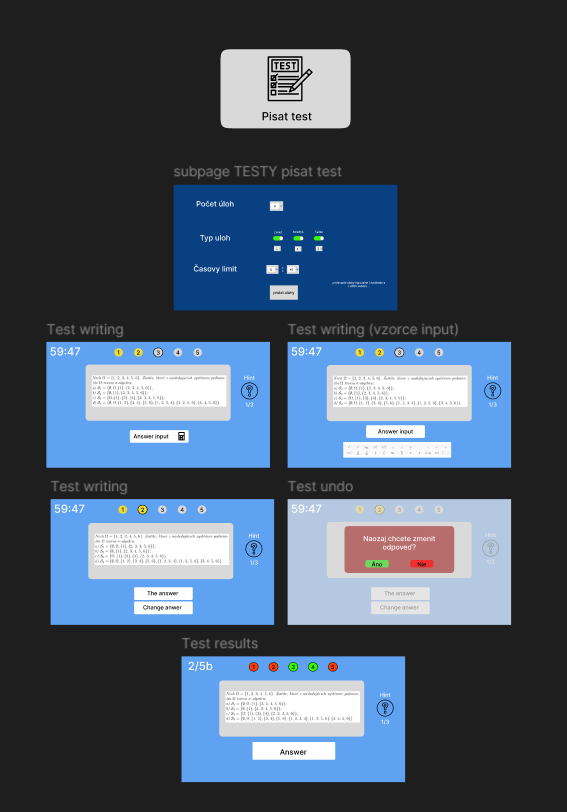
\includegraphics[width=16cm]{img/figma_screen.png}
  \caption{Výrez z konceptuálneho návrhu podstránky Písať test.}
  \label{figmavizual}
\end{figure} 

\subsection{Preskúšanie sa}

Súčasťou navrhovanej webovej aplikácie je stránka umožňujúca používateľom vytvárať vlastné testovacie sady úloh na precvičenie a preverenie vedomostí z oblasti pravdepodobnosti a štatistiky.
 Používateľské rozhranie tejto stránky (obrázok~\ref{test-creation}) bolo navrhnuté tak, aby bolo intuitívne a aby bola použivateľská skúsenosť čo najlepšia (\acrshort{ux}).

\begin{figure}[h!]
  \centering
  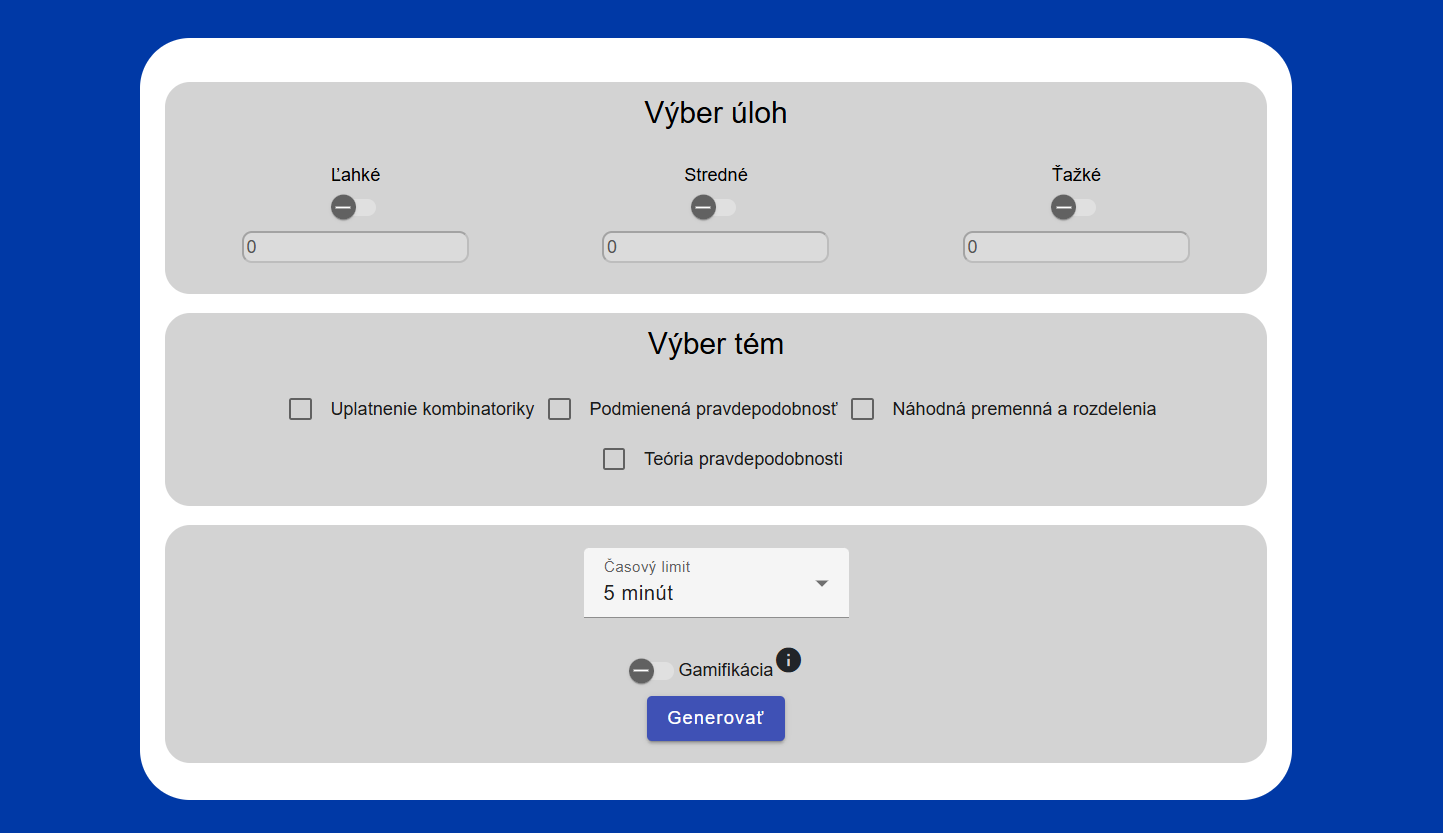
\includegraphics[width=14cm]{img/test-creation.png}
  \caption{Používateľské rozhranie stránky pre vytvorenie testovacej sady.}
  \label{test-creation}
\end{figure}

Na tejto stránke má používateľ možnosť presne definovať parametre generovaného testu, ako napríklad:

\begin{itemize}
  \item \textbf{Výber tém} – používateľ si môže označiť matematické témy, z ktorých chce byť testovaný. Ide najmä o témy ako pravdepodobnosť a rozdelenia, štatistika a analýza dát, kombinatorika a teória množín, a tiež aplikácie a reálne scenáre.
  \item \textbf{Typ a obtiažnosť úloh} – umožňuje nastaviť počet ľahkých, stredne ťažkých a ťažkých úloh.
  \item \textbf{Časový limit} – určuje maximálny čas na vypracovanie celého testu.
  \item \textbf{Gamifikácia} – voliteľná funkcionalita, ktorej účelom je zvýšiť motiváciu používateľov prostredníctvom herných prvkov, bližšie vysvetlená v nasledujúcej podkapitole.
\end{itemize}

Po úspešnom vygenerovaní testovej sady je používateľ automaticky presmerovaný na stránku samotného preskúšania (obrázok~\ref{test-writing}). 
Pri návrhu tejto stránky sme kládli dôraz na vizuálnu spätnú väzbu pre používateľa – už zodpovedané úlohy sú jasne vizuálne označené, čím sa zlepšuje prehľadnosť testu. 
Súčasťou rozhrania je aj stručný popis používania aplikácie, ktorý sa zobrazí kliknutím na príslušnú ikonu s informáciami.

Po uplynutí časového limitu sa používateľovi automaticky zobrazí modálne okno, ktoré informuje o ukončení testu a odoslaní odpovedí na spracovanie a vyhodnotenie.

Na správne a čitateľné vykresľovanie matematických výrazov a rovníc bola použitá JavaScriptová knižnica \textbf{MathJax}.
 Tá zabezpečuje bezproblémové zobrazenie matematických symbolov a vzorcov priamo vo webovom prehliadači používateľa.
\begin{figure}[h!]
  \centering
  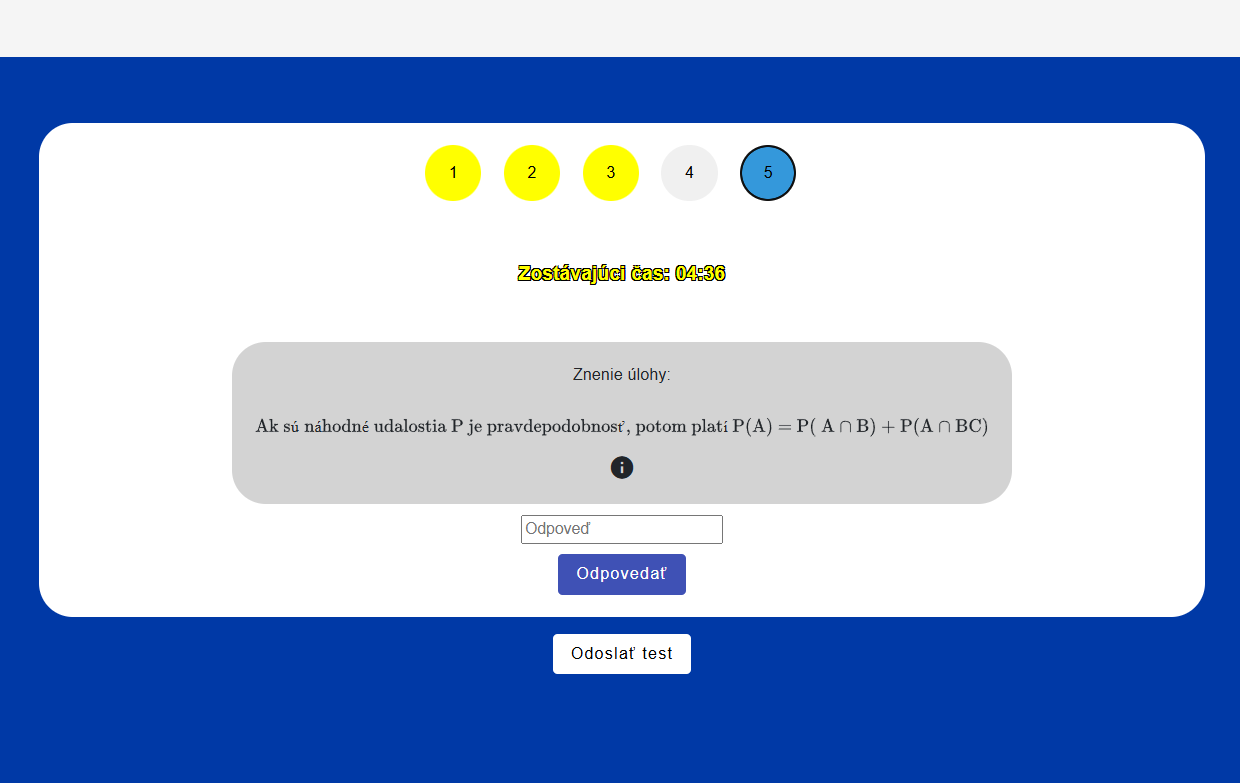
\includegraphics[width=14cm]{img/test-writing.png}
  \caption{Používateľské rozhranie stránky počas priebehu testu.}
  \label{test-writing}
\end{figure}



\subsubsection{Gamifikácia}

S cieľom zvýšiť atraktívnosť vzdelávacieho procesu a posilniť motiváciu študentov bola do aplikácie implementovaná \textbf{gamifikácia}, teda využitie herných prvkov v nehernom kontexte. 
Gamifikačné mechanizmy majú potenciál výrazne zlepšiť angažovanosť študentov, podporiť ich súťaživosť a vytvoriť pozitívne motivujúce prostredie na systematické precvičovanie vedomostí.

V rámci navrhnutej aplikácie sme zaviedli nasledujúce gamifikačné prvky:

\begin{itemize} \item \textbf{Percentilové hodnotenie} – namiesto klasického zoradenia používateľov podľa počtu bodov aplikácia využíva hodnotenie na základe \textbf{percentilu}. 
  Tento ukazovateľ vyjadruje, aké percento ostatných študentov dosiahlo horší alebo rovnaký výsledok.
   Zobrazenie percentilu poskytuje študentovi okamžitú a objektívnu informáciu o jeho relatívnej výkonnosti v rámci všetkých účastníkov testovania a zároveň ho motivuje k ďalšiemu zlepšovaniu.
  Ukážku zobrazovania percentilového hodnotenia možno vidieť na obrázku~\ref{test-results}.
  

\item \textbf{Bodový systém s bonusmi} – používateľ získava štandardné body za každú správne zodpovedanú otázku. 
Okrem toho sú prideľované aj bonusové body za rýchlosť odpovede, čím sa študenti podporujú v efektívnom a rýchlom riešení úloh.

\item \textbf{Vizuálna a zvuková spätná väzba} – aplikácia okamžite reaguje na správne alebo nesprávne odpovede študenta.
 Vizuálne je táto spätná väzba reprezentovaná farebným označením stavu jednotlivých otázok, pričom je doplnená aj vhodnými zvukovými efektmi. 
Týmto spôsobom dostáva používateľ jasnú a jednoznačnú informáciu o svojej aktuálnej úspešnosti. Čo je zobrazené na obrázku~\ref{gamification}.

\begin{figure}[H]
  \centering
  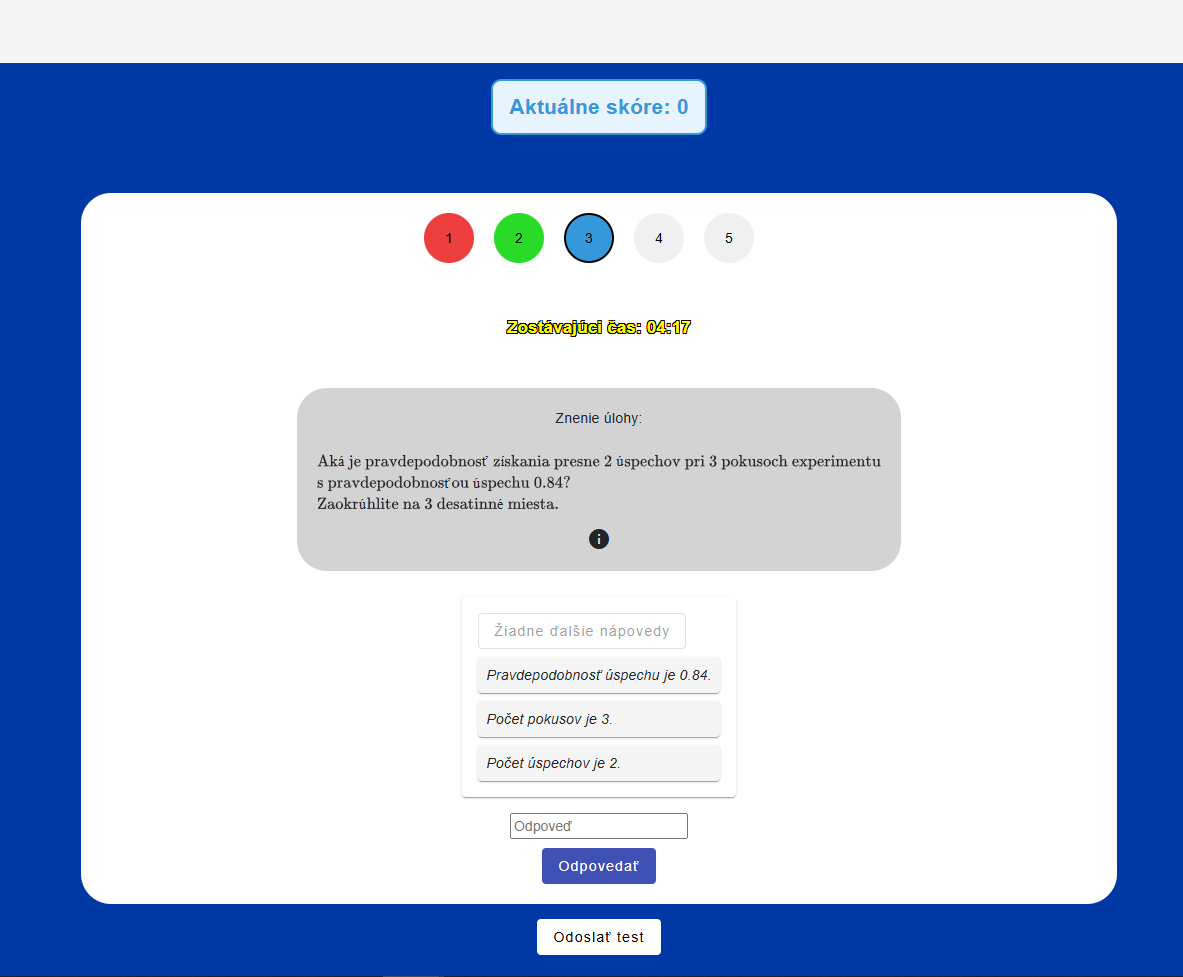
\includegraphics[width=14cm]{img/gamification.png}
  \caption{Ukážka vizuálnej spätnej väzby v gamifikovanom režime testovania.}
  \label{gamification}
\end{figure}

\item \textbf{Nápovedy s penalizáciou} – v prípade, že používateľ potrebuje pomôcť s riešením úloh, má možnosť využiť nápovedu. Tá ho môže nasmerovať k správnemu riešeniu, avšak za každú použitú nápovedu sú používateľovi odpočítané body. Týmto spôsobom podporujeme študentov k samostatnosti a zároveň pridávame do vzdelávania súťažný rozmer. \end{itemize}

Na stránke so štatistikami má študent následne možnosť vidieť, v akom percentile výkonnosti sa nachádza, čo mu poskytuje objektívnu informáciu o jeho relatívnej úspešnosti voči ostatným používateľom aplikácie. Tieto prvky spolu vytvárajú efektívne a interaktívne prostredie, ktoré podporuje kontinuálne vzdelávanie a rozvoj matematických schopností študentov.
\subsubsection{Generovanie úloh}

Pri návrhu aplikácie sme sa rozhodli implementovať mechanizmus \textbf{automatického generovania úloh}, ktorého cieľom bolo zvýšiť variabilitu testov a zabezpečiť, aby používatelia neboli limitovaní iba na statické úlohy uložené v databáze. 
Takto generované úlohy pridávajú do testovania prvok náhodnosti a prekvapenia, čím dochádza k efektívnejšiemu prevereniu skutočných vedomostí a schopností študenta.
Generátor úloh je navrhnutý tak, aby dynamicky vytváral nové zadania založené na vybraných pravdepodobnostných rozdeleniach. V súčasnej verzii aplikácie podporujeme generovanie úloh z nasledujúcich rozdelení:

\begin{itemize} \item \textbf{Binomické rozdelenie} \item \textbf{Geometrické rozdelenie} \item \textbf{Hypergeometrické rozdelenie} \item \textbf{Poissnovo rozdelenie} \item \textbf{Rovnomerné rozdelenie} \end{itemize}

Každá vygenerovaná úloha je unikátna, pričom vstupné parametre ako počet pokusov, počet úspechov alebo pravdepodobnosť úspechu sú generované náhodne v definovanom rozsahu.
\subsection{Materiály}
Ďalšou súčasťou aplikácie je sekcia študijných materiálov, ktorá slúži študentom ako podpora počas štúdia matematickej štatistiky a pravdepodobnosti. 
Táto časť aplikácie obsahuje systematicky usporiadané študijné poznámky, ktoré pokrývajú učebné osnovy predmetu Matematická štatistika.
 Obsah je kategorizovaný podľa jednotlivých tematických oblastí, a tak sa dá v študovanom obsahu jednoducho orientovať.

Každá téma obsahuje teoretické poznatky spolu s jasne spracovanými vzorovými príkladmi. 
Súčasťou týchto príkladov je aj detailný postup výpočtu, ktorý študentom slúži ako metodická pomôcka pri riešení podobných úloh.

\begin{figure}[H]
  \centering
  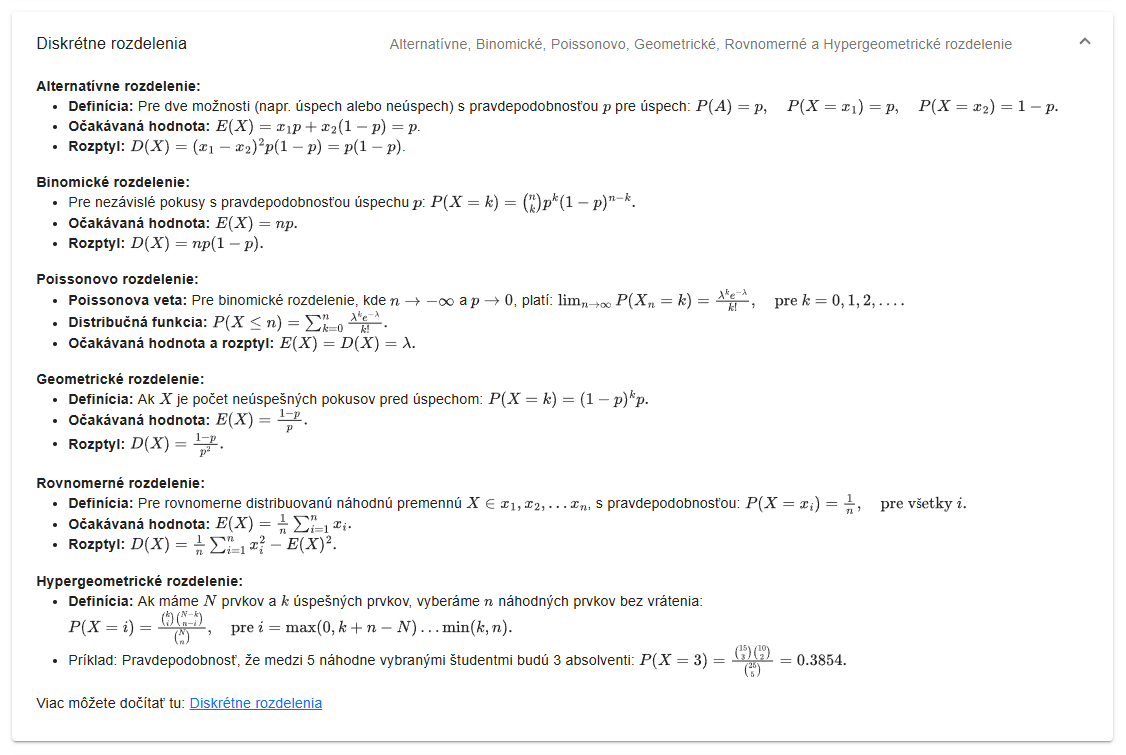
\includegraphics[width=14cm]{img/materialy.png}
  \caption{Ukážka sekcie študijných materiálov s príkladom.}
  \label{materialy}
  \end{figure}

\subsubsection{Interaktívne grafy}
Na zvýšenie interaktivity a pochopenia zložitých matematických konceptov sú v rámci materiálov integrované aj interaktívne grafy. 
Tieto grafy vizuálne demonštrujú dôležité pravdepodobnostné princípy, ako napríklad priebehy distribučných funkcií alebo hustoty pravdepodobnosti rôznych rozdelení. 
Grafické znázornenie výrazne uľahčuje študentom pochopenie abstraktných matematických myšlienok a prehlbuje ich schopnosť aplikovať získané vedomosti v praxi.
\begin{figure}[H]
  \centering
  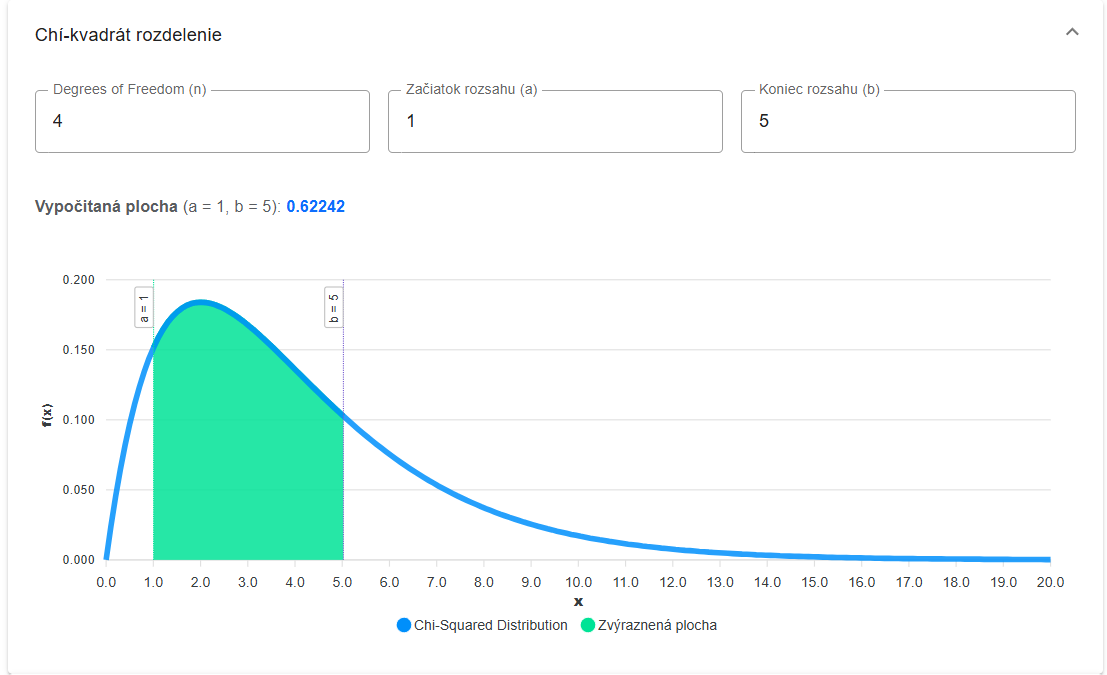
\includegraphics[width=14cm]{img/grafy.png}
  \caption{Ukážka interaktívneho grafu.}
  \label{grafy}
  \end{figure}

\subsection{Vyhodnocovanie úloh}

Po dokončení testu má používateľ k dispozícii detailný rozbor svojho riešenia. 
Na tejto podstránke je možné spätne prehliadať absolvované testy, pričom ku každému testu je zobrazovaný zoznam jednotlivých úloh s vyznačením správnosti odpovede.

 Každú úlohu je možné rozkliknúť a prezrieť si zadanie spolu s odpoveďou, čo podporuje proces spätného učenia a upevňovania vedomostí.

Okrem samotného zoznamu úloh je súčasťou zobrazenia aj základné štatistické zhrnutie testu, ako napríklad počet správnych odpovedí, celkový počet získaných bodov a dosiahnutý percentil.

Percentil poskytuje používateľovi okamžitú informáciu o jeho relatívnom postavení medzi všetkými účastníkmi testovania, a to na základe získaného skóre.


\begin{figure}[H]
  \centering
  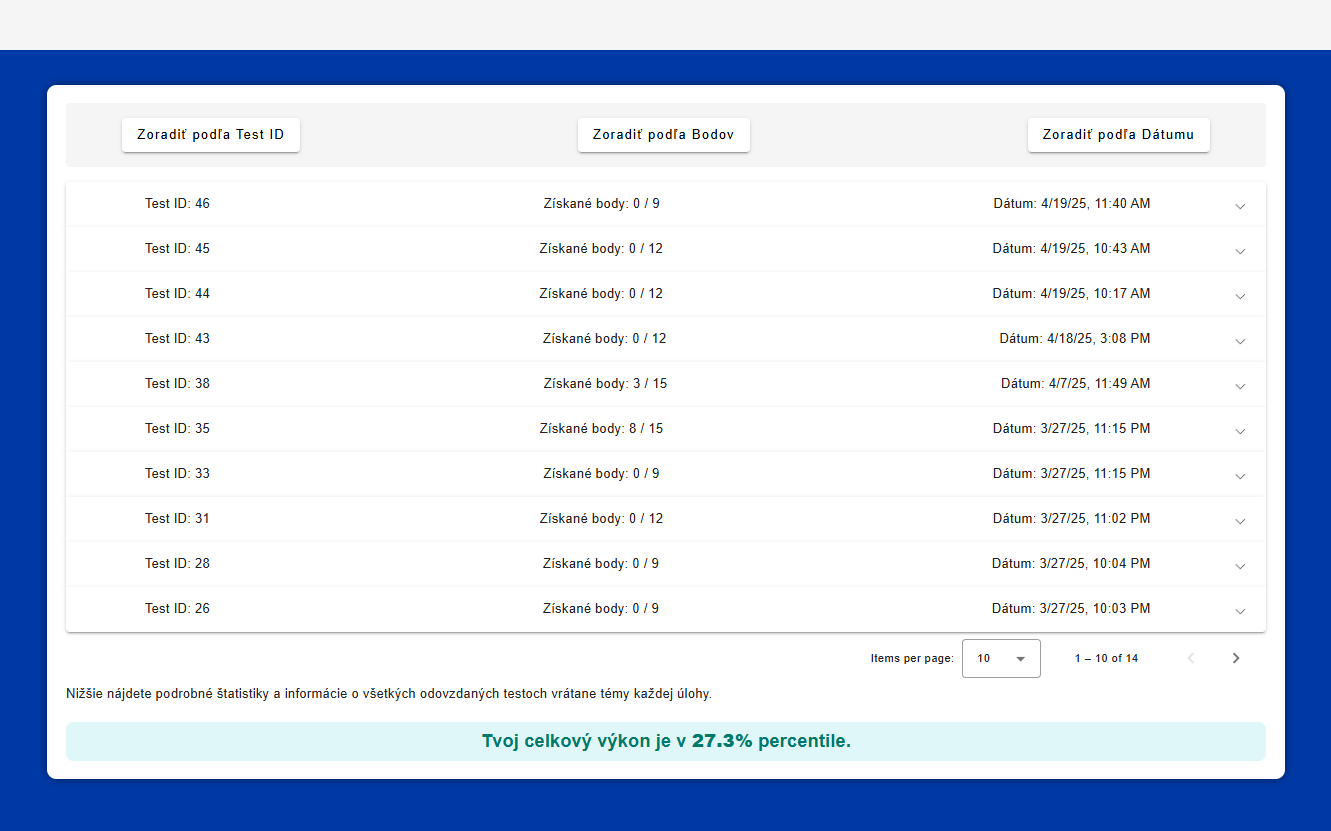
\includegraphics[width=14cm]{img/test-results.png}
  \caption{Ukážka podstránky vyhodnocovania testu a zobrazenie dosiahnutého percentilu.}
  \label{test-results}
\end{figure}



\subsection{Vytváranie a úprava úloh administrátorom}

V rámci administrátorskej časti aplikácie bola implementovaná funkcionalita umožňujúca správcom systému vytvárať nové úlohy a upravovať existujúce zadania.
 Cieľom tejto funkcionality je umožniť dynamické rozširovanie databázy úloh bez potreby manuálnych zásahov do databázy na úrovni servera.

Pri návrhu rozhrania na vkladanie úloh bolo dôležité zabezpečiť, aby bol proces tvorby matematických otázok intuitívny a používateľsky prívetivý, najmä pri práci s matematickými zápismi a vzorcami.
 Tento cieľ bol dosiahnutý integráciou knižnice \textbf{MathQuill}, ktorá umožňuje dynamické a interaktívne zadávanie matematických výrazov.

\textbf{MathQuill} poskytuje rozhranie, v ktorom môže administrátor zadávať matematické vzorce v LaTeX formáte. 
V reálnom čase dochádza k ich prekladu do vizuálne čitateľnej podoby, čím sa zabezpečuje okamžitá spätná väzba a minimalizácia syntaktických chýb.
 Matematické výrazy sú zobrazované v editovateľnom textovom poli, ktoré verne imituje klasickú matematickú notáciu, čo výrazne zvyšuje používateľský komfort a presnosť zadávania úloh.

Táto funkcionalita nielen zjednodušuje proces tvorby úloh, ale zároveň zaručuje, že všetky matematické zápisy budú správne interpretované pri zobrazovaní úloh študentom v testoch a materiáloch.

\begin{figure}[H]
  \centering
  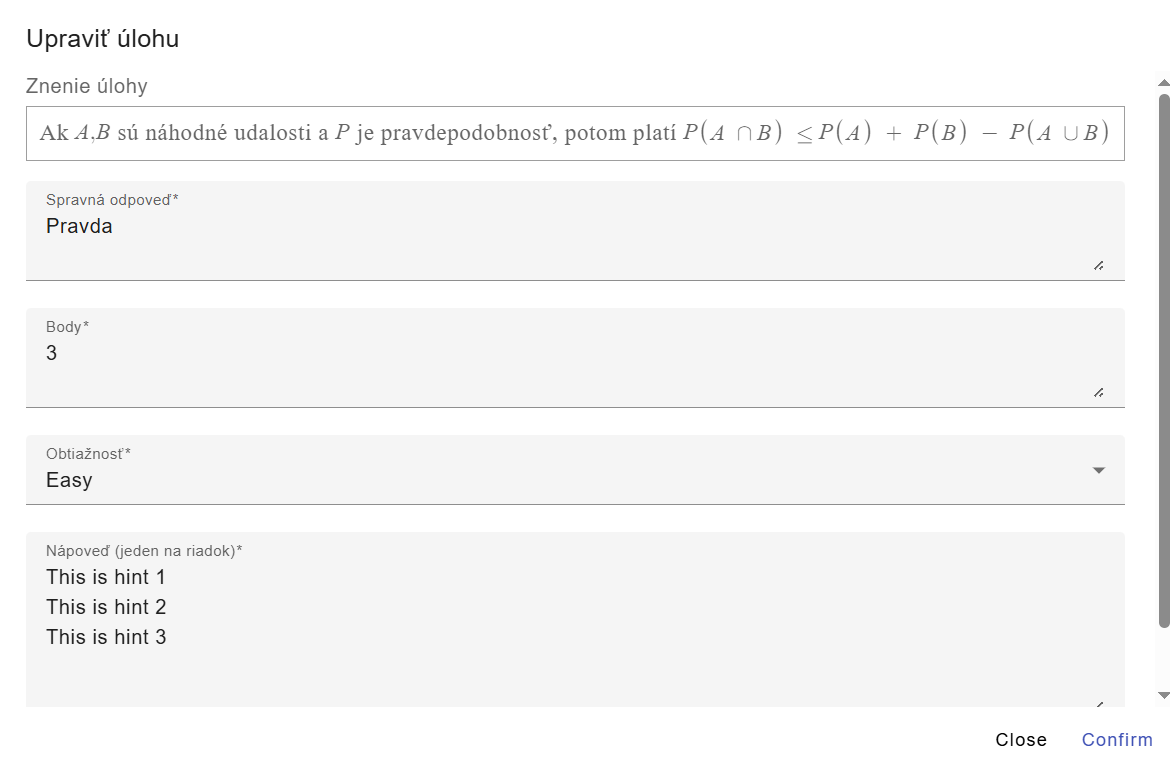
\includegraphics[width=14cm]{img/edit_ulohy.png}
  \caption{Ukážka administrátorského rozhrania na úpravu úloh.}
  \label{fig:admin_edit}
\end{figure}

Na obrázku \ref{fig:admin_edit} je možné vidieť instantný preklad pomocou knižnice MathQuill pri editovaní úlohy. Používateľ zadáva výraz v LaTeX formáte, ktorý sa okamžite zobrazí vo vykreslenej matematickej forme.

Použitý zápis:
\begin{lstlisting}[style=code-listing, caption={LaTeX zápis matematického výrazu}]
\begin{aligned}
    & \text{Nech }X\sim N(4,1). \text{Nájdite }a\text{ tak, že }P(2X+1\le a)=0.9. \\
    & \textbf{Odpoveď zapíšte ako desatinné číslo zaokrúhlené na štyri desatinné miesta.}
    \end{aligned}  \end{lstlisting}
  

\subsection{Export testov a výsledkov}

V rámci rozšírenia funkcionality aplikácie bola implementovaná sekcia \textbf{Export}, ktorá reflektuje potreby a preferencie študentov preferujúcich tradičné metódy učenia, ako je štúdium pomocou papiera a pera aj v digitálnej ére.

Stránka Export obsahuje dve hlavné funkcionality:

\begin{itemize}
    \item \textbf{Generovanie testu do PDF formátu} – používateľ má možnosť vygenerovať si novú sadu úloh podobne ako v režime preskúšania.
     Úlohy sú obohatené o nápovedy a následne spracované do PDF dokumentu, ktorý si študent môže vytlačiť a riešiť v offline prostredí.
      Táto funkcionalita je určená najmä pre tých, ktorí uprednostňujú fyzický výpočet úloh a písanie riešení na papier.

    \item \textbf{Export vypracovaných výsledkov} – študent si môže stiahnuť aj prehľad svojich absolvovaných testov vrátane odpovedí, výsledkov a štatistík.
     Tento export umožňuje jednoduchú archiváciu pokroku a spätnú analýzu riešených úloh.
\end{itemize}

Obe PDF súbory sú generované dynamicky na základe dát získaných z aplikácie, pričom na tvorbu dokumentov je využívaná knižnica \textbf{pdfmake}.
 Štruktúra vygenerovaných súborov bola navrhnutá tak, aby bola prehľadná, čitateľná a používateľsky prívetivá.

Na obrázku~\ref{pdf-export} je ukážka časti vygenerovaného PDF dokumentu obsahujúceho zadania úloh.

\begin{figure}[h!]
  \centering
  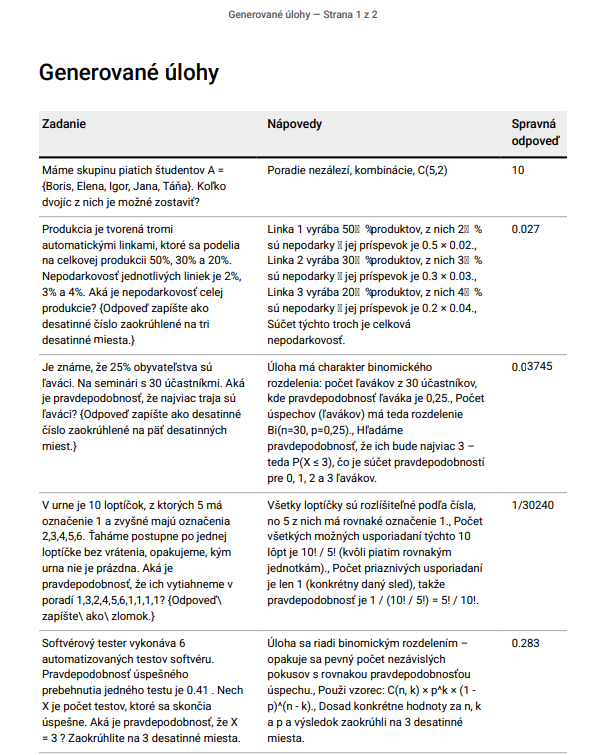
\includegraphics[width=14cm]{img/pdf.png}
  \caption{Ukážka vygenerovaného PDF súboru so sadou úloh na precvičovanie.}
  \label{pdf-export}
\end{figure}


 \section{Implementácia webovej aplikácie}
 V tejto kapitole sa podrobne venujeme implementačnej časti webovej aplikácie, pričom rozdeľujeme jednotlivé aspekty systému na backend, frontend a databázovú vrstvu.
  Cieľom tejto časti je ukázať, ako boli teoretické návrhy z predchádzajúcej kapitoly pretavené do konkrétnej technickej realizácie.

 V jednotlivých sekciách prezentujeme použité technológie a knižnice, ako aj konkrétne časti zdrojového kódu ilustrujúce dôležité funkcionality, 
 ako napríklad generovanie úloh, vizualizácie dát pomocou grafov alebo spracovanie používateľského vstupu pri pridávaní nových otázok do databázy.

 \subsection{Vývojové prostredie a inštalácia závislostí}

 Počas vývoja webovej aplikácie sme využívali vývojové prostredie \textbf{Visual Studio Code}\cite{vscode}, ktoré poskytuje množstvo rozšírení vhodných pre vývoj v JavaScripte a TypeScripte, ako aj nástroje na efektívnu správu projektovej štruktúry, ladenie a kontrolu syntaxe.
 
 Backendová časť aplikácie bola postavená na platforme \textbf{Node.js}, ktorá umožňuje spúšťanie JavaScriptového kódu na strane servera. Na správu knižníc a závislostí sme používali \acrfull{npm}, ktorý je súčasťou štandardnej inštalácie Node.js. 
 Pomocou neho boli do projektu inštalované všetky potrebné knižnice, ako napríklad \texttt{express}, \texttt{MathQuill}, \texttt{body-parser}, \texttt{cors} a ďalšie.
  
 Závislosti boli definované v súbore \texttt{package.json}, ktorý slúži zároveň ako dokumentačný a konfiguračný súbor pre projekt. Samotná inštalácia všetkých závislostí sa vykoná príkazom:
 
 \begin{verbatim}
 npm install
 \end{verbatim}
 
 Týmto príkazom sa automaticky stiahnu všetky knižnice uvedené v súbore \texttt{package.json} a pripravia sa na použitie v projekte.
 
 \subsection{Frontend – Angular }

Frontendová časť aplikácie bola implementovaná pomocou frameworku \textbf{Angular}, ktorý je postavený na TypeScripte a poskytuje robustnú architektúru pre budovanie komplexných single-page aplikácií (SPA).
 Angular ponúka množstvo výhod ako je komponentovo orientovaný vývoj, dvojcestná väzba dát, modulárnosť a rozsiahla komunita s kvalitnou dokumentáciou.

\bigskip
Na to, aby sme mohli Angular používať, je potrebné mať nainštalovaný \textbf{Node.js} a s ním aj správcu balíkov \acrshort{npm}, ktoré sme spomínali v predchádzajúcej sekcii. 
Po ich nainštalovaní je možné Angular \acrshort{cli} nainštalovať globálne\footnote{Prepínač \textit{-g} znamená globálnu inštaláciu, čím získame prístup ku príkazu \textit{ng} v ktoromkoľvek priečinku systému.}
pomocou príkazu:

\begin{verbatim}
npm install -g @angular/cli
\end{verbatim}

Správnu inštaláciu Angularu môžeme overiť pomocou príkazu:

\begin{verbatim}
ng version
\end{verbatim}

Výstup z tohto príkazu zobrazí verziu Angular \acrshort{cli}, ako aj verzie jednotlivých komponentov Angularu. Na obrázku~\ref{fig:ng-version} je znázornený výstup z tohto príkazu v termináli\footnote{Terminál vo Visual Studio Code predstavuje integrované rozhranie pre prácu s príkazovým riadkom priamo v editore.}.

\begin{figure}[H]
  \centering
  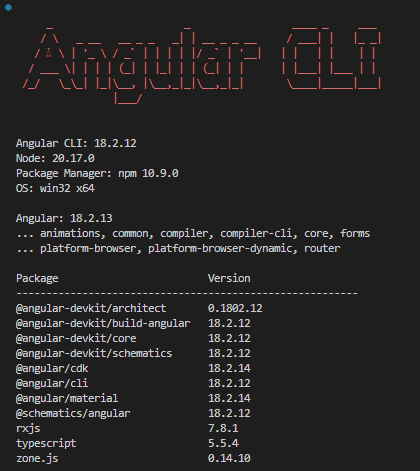
\includegraphics[width=10cm]{img/ng-version.png}
  \caption{Výstup príkazu \texttt{ng version} v termináli.}
  \label{fig:ng-version}
\end{figure}

\bigskip
Nový Angular projekt môžeme vytvoriť pomocou príkazu:

\begin{verbatim}
ng new angular-app
\end{verbatim}

Tento príkaz vygeneruje základnú adresárovú štruktúru aplikácie, vrátane konfiguračných súborov, ako je napríklad \texttt{angular.json}, \texttt{package.json}, a priečinkov \texttt{src/}, \texttt{app/} a ďalších. Po úspešnom vytvorení projektu môžeme aplikáciu spustiť príkazom:

\begin{verbatim}
ng serve --port 80
\end{verbatim}

Týmto príkazom sa automaticky nainštalujú všetky závislosti zo súboru \texttt{package-lock.json} a vytvorí sa priečinok \texttt{node\_modules}, ktorý obsahuje všetky knižnice potrebné na beh aplikácie.
 Aplikácia je následne dostupná na adrese \texttt{http://localhost:80}.

Na obrázku~\ref{fig:angular-structure} je znázornená základná adresárová štruktúra Angular projektu po vytvorení, pričom na obrázku~\ref{fig:project-structure} je zobrazená štruktúra nášho projektu.

\begin{figure}[H]
  \centering
  \begin{minipage}[t]{0.48\textwidth}
    \centering
    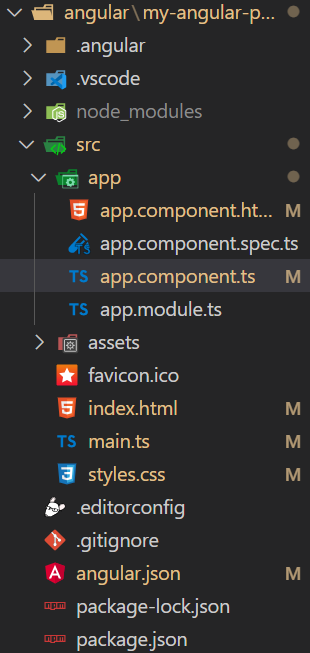
\includegraphics[width=\linewidth]{img/angular-structure.png}
    \caption{Základná štruktúra Angular projektu.}
    \label{fig:angular-structure}
  \end{minipage}
  \hfill
  \begin{minipage}[t]{0.48\textwidth}
    \centering
    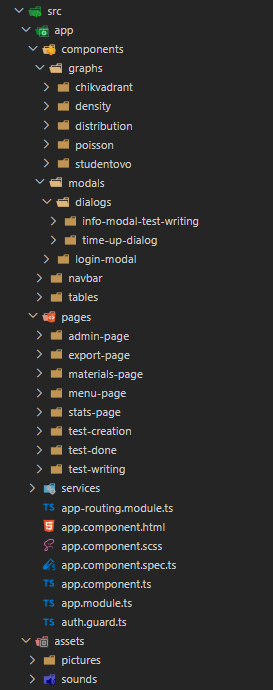
\includegraphics[width=\linewidth]{img/project-structure.png}
    \caption{Naša štruktúra projektu.}
    \label{fig:project-structure}
  \end{minipage}
\end{figure}


\subsubsection{Implementácia grafickej časti}
Pri implementácii grafického rozhrania webovej aplikácie sme kládli dôraz na jednotný vzhľad, prehľadnosť a používateľskú prívetivosť.
 Aby sme zabezpečili konzistentnosť vzhľadu naprieč celou aplikáciou, rozhodli sme sa použiť knižnicu \textbf{Angular Material}.
  Táto knižnica poskytuje súbor preddefinovaných UI komponentov a interaktívnych prvkov v súlade s dizajnovým jazykom Material Design, čím výrazne zjednodušuje vývoj a zároveň zachováva estetickú konzistenciu.

Integrácia knižnice Angular Material do aplikácie prebiehala jednoduchým príkazom:

\begin{verbatim}
  ng add @angular/material
\end{verbatim}

Ako doplnkovú technológiu sme použili \textbf{node-sass}, čo je nástroj umožňujúci kompiláciu súborov \acrshort{scss} do štandardných \acrshort{css} súborov.
 Tento nástroj podporuje pokročilé \acrshort{css} techniky, ako napríklad vnorenie pravidiel, používanie premenných a mixinov\footnote{Mixiny sú opakovateľné skupiny štýlov v SCSS, ktoré zjednodušujú kód.}, čím je zabezpečené efektívnejšie spravovanie štýlov celej aplikácie.

 Zvukové prvky, ktoré dopĺňajú herné mechanizmy gamifikácie, boli integrované prostredníctvom platformy \textbf{Freesound.org}\cite{freesong}, ktorá poskytuje verejne dostupné zvukové efekty.
 
 \subsubsection{Vizualizácia matematických výrazov pomocou MathJax }
 Na vizualizáciu matematických výrazov sme v našej aplikácii použili JavaScriptovú knižnicu \textbf{MathJax}. 
 Knižnicu sme zvolili pre jej schopnosť efektívne a presne zobrazovať rôzny matematický obsah, ako sú zápisy, vzorce alebo rovnice. 
 Jednoduché vykreslenie matematiky napísanej v LaTeX formáte priamo v \acrshort{html} elementoch vykonáva MathJax pomocou špeciálnej property:

\begin{verbatim}
 <p [mathjax]="$$content$$"></p>
  \end{verbatim}
 Týmto spôsobom MathJax automaticky preloží LaTeX zápis do vizuálne čitateľnej matematickej podoby priamo v prehliadači používateľa a matematický zápis sa zobrazí dynamicky, bez ďalšej potreby iných manuálnych zásahov do \acrshort{dom} stromu.

  \begin{figure}[H]
    \centering
    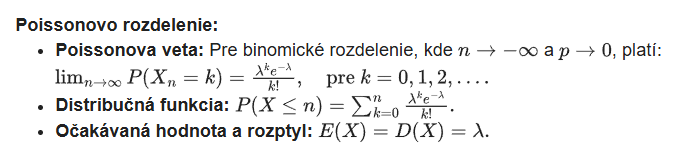
\includegraphics[width=13cm]{img/mathjax_priklad.png}
    \caption{Ukážka zobrazenia matematického výrazu pomocou MathJax.}
    \label{fig:mathjax-priklad}
  \end{figure}

  \subsubsection{Zadávanie matematických výrazov s MathQuill}

 Pri voľbe knižnice vhodnej na zadávanie matematických výrazov sme kládli dôraz na to, aby bol spôsob zadávania pre administrátora intuitívny a používateľský jednoduchý.
 Z tohto dôvodu sme zvolili knižnicu \textbf{MathQuill}, ktorá umožňuje administrátorovi zapisovať matematiku v reálnom čase pomocou LaTeX syntaxe, ktorá sa po zapísaní okamžite vizuálne prekladá do štandardného matematického zápisu.
 Pri riešení problematiky zadávania matematických výrazov, sme využili aj výhody knižnice \textbf{jQuery}, na ktorej je MathQuill závislá.
 Knižnica jQuery zabezpečuje asynchrónnu manipuláciu s \acrshort{html} a \acrshort{css} prvkami stránky,  a jednoduchú prácu s animáciami a \acrshort{dom} elementmi.
 Spojením týchto technológií sme vytvorili plynulé a responzívne prostredie, dokonalo vhodné na prácu s matematickými výrazmi.

 \subsection{Export úloh do PDF formátu pomocou pdfmake}

 Exportná stránka našej aplikácie disponuje funkciou generovania PDF dokumentu, ktorý obsahuje súhrn úloh, ich správnych odpovedí a prípadných nápoved.
 Na vytvorenie tejto funkcie sme využili knižnicu \textbf{pdfmake}, ktorá bola do projektu integrovaná pomocou nasledovného príkazu:  
 \begin{verbatim} npm install pdfmake \end{verbatim}
 
PDF dokument sa vytvorí zostavením tzv. \texttt{documentDefinition} objektu, ktorý definuje rozloženie, obsah a štýl dokumentu.
 Do dokumentu sa následne vloží tabuľka dynamicky vygenerovaných úloh, pričom každá úloha bude vyzobrazená v jednom riadku tabuľky.
 
 Ukážka definície hlavičky a štýlu tabuľky:
 
 \begin{lstlisting}[ caption={Zjednodušená štruktúra PDF dokumentu}, label={lst:pdf-header}, language=java, style=code-listing ] 
  const documentDefinition = { 
    pageSize: 'A4', 
    header: (currentPage, pageCount) => ({ 
      text: Generované úlohy - Strana ${currentPage} z ${pageCount}, 
      alignment: 'center', 
      style: 'header' }), 
      content: [ { 
        table: { headerRows: 1, 
        widths: ['auto', 'auto', ''], 
      body: [ ['Zadanie', 'Nápovedy', 'Správna odpoveď'],
      ...this.exercises.map(ex => [ ... ]) ] 
              } 
        } ],
       styles: { / ... */ } }; 
      
      \end{lstlisting}
 
 Keďže zadania úloh obsahujú matematické výrazy vo formáte LaTeX, pred ich vložením do PDF je potrebné ich vyčistiť od LaTeX príkazov. Túto úlohu rieši pomocná funkcia:
 
 \begin{lstlisting}[ caption={Odstránenie LaTeX syntaxe zo zadania úlohy}, label={lst:latex-cleaner}, language=java, style=code-listing ] 
  function removeLatexCommands(text) { 
    text = text.replace(/\text{([^}]*)}/g, '$1');
    return text.replace(/\[a-zA-Z]+/g, '').trim(); 
   }
   \end{lstlisting}
 
 Výsledný PDF dokument je vytvorený pomocou volania služby: 
 
 \texttt{pdfMake.createPdf(documentDefinition).download('...');}
 
 Na obrázku~\ref{pdf-export} je uvedený príklad takto vygenerovaného výstupu.
\subsection{Vizualizácia dát pomocou ApexCharts}

Na vizualizáciu dát a grafických zobrazení v rámci aplikácie sme zvolili knižnicu \textbf{ApexCharts}. 
Grafy, ktoré táto knižnica poskytuje, sú moderné, responzívne a ľahko implementovateľné pre Angular aplikácie.
 Integrovali sme ju nasledovným jednoduchým príkazom v termináli: 
 
 \begin{verbatim} npm install apexcharts ng-apexcharts \end{verbatim}
 
 Po úspešnej inštalácii balíkov je možné vytvoriť požadované grafy priamo v komponente aplikácie. 
 Ako konkrétny príklad uvádzame vizualizáciu hustoty pravdepodobnosti \textbf{Chí-kvadrát rozdelenia}, ktorého implementáciu máme zahrnutú aj vo vizuálnej časti tejto práce (viď obrázok č.~\ref{grafy}).
 
 Výpočet jednotlivých bodov pre vykreslenie Chí-kvadrát rozdelenia realizujeme nasledovnou metódou:
 
 \begin{lstlisting}[ caption={Výpočet bodov Chí-kvadrát rozdelenia}, label={lst:chikvadrat-distribution}, language=java, style=code-listing ] 
  calculateChiSquared(degreesOfFreedom: number): { x: number; y: number }[] {
    const gamma = (z: number): number => {
      if (z === 1) return 1;
      if (z === 0.5) return Math.sqrt(Math.PI);
      return (z - 1) * gamma(z - 1);
    };

    const chiPDF = (x: number, df: number): number => {
      if (x <= 0) return 0;
      const k = df / 2;
      const numerator = Math.pow(x, k - 1) * Math.exp(-x / 2);
      const denominator = Math.pow(2, k) * gamma(k);
      return numerator / denominator;
    };

    const chiData = [];
    const maxRange = 20;
    const step = 0.1;

    for (let x = 0; x <= maxRange; x += step) {
      chiData.push({
        x: parseFloat(x.toFixed(1)),
        y: parseFloat(chiPDF(x, degreesOfFreedom).toFixed(4)),
      });
    }

    return chiData;
  } 

\end{lstlisting}

Takto pripravené dáta sú následne vizualizované pomocou komponentu \texttt{apx-chart}, ktorý implementujeme priamo do HTML šablóny Angular komponentu nasledovne:

\begin{lstlisting}[ caption={Vykreslenie grafu v šablóne pomocou ApexCharts}, label={lst:apexchart-usage}, language=HTML, style=code-listing ]
  
  <apx-chart 
   [series]="chiChartOptions.series || []" 
   [chart]="chiChartOptions.chart || { type: 'line' }" 
   [xaxis]="chiChartOptions.xaxis || {}" 
   [yaxis]="chiChartOptions.yaxis || {}" 
   [markers]="chiChartOptions.markers || {}" 
   [annotations]="chiChartOptions.annotations || {}"> 
   </apx-chart> 

  \end{lstlisting}

Týmto prístupom sme v aplikácii dosiahli efektívnu a jednoduchú implementáciu grafických vizualizácií pravdepodobnostných rozdelení a ponúkli sme používateľom možnosť intuitívnejšieho pochopenia zložitých matematických konceptov.

Na optimalizáciu výkonu pri práci s grafmi sme implementovali oneskorené vykresľovanie (lazy-loading) pomocou Angular direktívy \texttt{*ngIf}. 
Komponenty s grafmi sa inicializujú až v momente, keď používateľ otvorí príslušný obsah (napr. rozbaľovací panel \texttt{mat-expansion-panel}).
 Tento prístup efektívne znižuje čas načítania stránky a šetrí systémové prostriedky, pretože grafy sa nevytvárajú skôr, ako je to potrebné.
 

\subsection{Backend}
 Inštalácia a použitie Express frameworku
 \newline

Inštalácia Expressu je jednoduchá a vykonáva sa pomocou balíčkovacieho nástroja \acrshort{npm} príkazom:

\begin{verbatim} npm install express \end{verbatim}

Po úspešnej inštalácii je možné vytvoriť základný server a definovať vlastné API routy. Najjednoduchšia implementácia servera môže vyzerať nasledovne:

\begin{lstlisting}[ caption={Ukážka základnej konfigurácie Express.js servera}, label={lst:basic-express-server}, language=java, style=code-listing ] 
  const express = require('express'); 
  const app = express(); 
  const port = 3000;

app.listen(port, () => { console.log(Server beží na porte ${port}); }); 
\end{lstlisting}

Tento server môžeme spustiť cez terminál pomocou príkazu:

\begin{verbatim} node server.js \end{verbatim}

kde \texttt{server.js} je názov súboru obsahujúceho uvedený kód. Ak je server úspešne spustený, v konzole sa vypíše správa \uv{Server beží na porte 3000}.
 V projekte je logika rozdelená do tzv. \textbf{servisných tried} (services), ktoré abstrahujú jednotlivé domény funkcionality – napríklad práca s testami, používateľmi alebo štatistikami. 
 Tieto triedy slúžia ako rozhranie medzi routou a databázovou logikou. 
Na obrázku~\ref{fig:backend-services} je znázornený výrez zo štruktúry backendu so zameraním na jednotlivé služby.

Tento kód vytvorí základný server, ktorý je pripravený na ďalšie definovanie rout a pridávanie funkcionality.
 V projekte je logika rozdelená do tzv. \textbf{servisných tried} (services), ktoré abstrahujú jednotlivé domény funkcionality.
  Tieto triedy slúžia ako rozhranie medzi routou a databázovou logikou.
\begin{figure}[H]
  \centering
  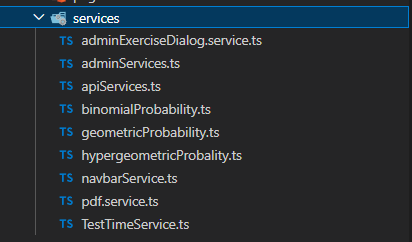
\includegraphics[width=13cm]{img/backend-services.png}
  \caption{Ukážka štruktúry backendových služieb v aplikácii.}
  \label{fig:backend-services}
\end{figure}

\bigskip
Na to, aby frontend mohol komunikovať s backendom, je potrebné povoliť prístup medzi rôznymi doménami (napr. frontend beží na \texttt{http://localhost:4200} a backend na \texttt{http://localhost:3000}). Na tento účel sme použili knižnicu \textbf{CORS} (\textit{Cross-Origin Resource Sharing}), ktorá bola nakonfigurovaná nasledovne:

\begin{lstlisting}[
  caption={Konfigurácia CORS pre komunikáciu medzi FE a BE},
  label={lst:cors-config},
  language=java,
  style=code-listing
]
const cors = require('cors');
app.use(cors({
  origin: 'http://localhost:4200',
  credentials: true
}));
\end{lstlisting}

Bez tejto konfigurácie by prehliadač blokoval požiadavky medzi rôznymi portmi alebo doménami, čo by znemožnilo komunikáciu medzi frontendom a backendom.

\bigskip
Na správne spracovanie dát typu \texttt{application/json}, ktoré odosiela Angular prostredníctvom POST alebo PUT požiadaviek, sme použili middleware \textbf{body-parser}. Tento middleware sa postará o to, že JSON objekt v tele požiadavky bude automaticky spracovaný a dostupný cez \texttt{req.body}. Je to obzvlášť dôležité pri práci s databázou PostgreSQL, kde používame dátový typ \texttt{JSONB}.

\begin{lstlisting}[
  caption={Použitie body-parser pre spracovanie JSON požiadaviek},
  label={lst:body-parser},
  language=java,
  style=code-listing
]
const bodyParser = require('body-parser');
app.use(bodyParser.json());
\end{lstlisting}

Týmto nastavením zabezpečíme, že každý JSON payload zo strany klienta bude backendom správne spracovaný a následne uložený do databázy vo formáte \texttt{JSONB}.


 \subsubsection{Autentifikácia}

 Prihlasovanie používateľov v aplikácii je riešené pomocou \textbf{LDAP autentifikácie}, pričom aplikácia komunikuje s akademickým LDAP serverom \texttt{ldap.stuba.sk}. Na overenie prihlasovacích údajov využívame knižnicu \texttt{ldap-authentication}, ktorá zabezpečuje jednoduché pripojenie a autentifikáciu voči vzdialenému LDAP serveru. Knižnica má ako závislosť \texttt{ldapjs}, ktorá realizuje nízkoúrovňovú komunikáciu.
 
 Samotná autentifikácia je realizovaná pomocou nasledovnej asynchrónnej funkcie:
 
 \begin{lstlisting}[
   caption={Funkcia na autentifikáciu používateľa cez LDAP},
   label={lst:ldap-auth},
   language=java,
   style=code-listing
 ]
 async function ldapAuth(username, password) {
   try {
     const options = {
       ldapOpts: { url: 'ldap://ldap.stuba.sk' },
       userDn: `uid=${username},ou=People,dc=stuba,dc=sk`,
       userPassword: password,
       userSearchBase: 'ou=People,dc=stuba,dc=sk',
       usernameAttribute: 'uid',
       username: username,
     };
 
     return await authenticate(options);
   } catch (error) {
     throw new Error('LDAP bind failed: ' + error.message);
   }
 }
 \end{lstlisting}
 
 Na strane backendu používame knižnicu \texttt{express-session}, ktorá nám umožňuje uchovávať informáciu o prihlásenom používateľovi v rámci session. Týmto spôsobom vieme zabezpečiť, že používateľ ostane prihlásený aj pri opakovanej návšteve stránky počas aktívnej relácie.
 
 Po úspešnej autentifikácii sa vytvorí zjednodušený objekt používateľa, ktorý sa uloží do databázy (ak ešte neexistuje), a zároveň sa uloží do session nasledovne:
 
 \begin{lstlisting}[
   caption={Spracovanie prihlasovania a uloženie používateľa do session},
   label={lst:login-session},
   language=java,
   style=code-listing
 ]
 app.post('/login', async (req, res) => {
   const { username, password } = req.body;
   try {
     const user = await ldapAuth(username, password);
     const processedUser = {
       userId: user.uisId,
       employeeType: user.employeeType,
       givenName: user.givenName,
       lastName: user.sn,
       email: user.mailLocalAddress[1],
     };
 
     // Insert into DB if new
     try {
       const existing = await db.findUserById(processedUser.userId);
       if (!existing) {
         await db.insertUser(processedUser);
       }
     } catch (dbErr) {
       console.error('DB error:', dbErr.message);
     }
 
     // Save user to session
     req.session.user = processedUser;
     res.status(200).json(processedUser);
   } catch (err) {
     res.status(401).json({ error: 'Authentication failed: ' + err.message });
   }
 });
 \end{lstlisting}
 
 \paragraph{Ochrana súkromných a administrátorských rout na strane frontendu}

Na strane klienta (v Angulari) využívame vlastný súbor \texttt{auth.guard.ts}, ktorý zaisťuje, že k určitým stránkam aplikácie má prístup iba autentifikovaný používateľ. Tento guard je súčasťou smerovania (routing) a overuje, či existuje používateľ v úložisku \texttt{sessionStorage}. Ak nie, používateľ je automaticky presmerovaný na prihlasovaciu stránku.

Okrem toho tento guard podporuje aj kontrolu rolí používateľov. Pomocou atribútu \texttt{expectedEmployeeType} v definícii trasy vieme zabezpečiť, že niektoré stránky (napr. administrátorské) budú dostupné len používateľom s určitou rolou (napr. \texttt{admin}).

\begin{lstlisting}[
  caption={Implementácia AuthGuard v Angulari},
  label={lst:auth-guard},
  language=java,
  style=code-listing
]
canActivate(route: ActivatedRouteSnapshot, state: RouterStateSnapshot): boolean {
  const user = this.apiService.getUserFromStorage();

  if (!user) {
    this.router.navigate(['/']);
    return false;
  }

  const expectedEmployeeType = route.data['expectedEmployeeType'];
  if (expectedEmployeeType && user.employeeType !== expectedEmployeeType) {
    this.router.navigate(['/menu']);
    return false;
  }

  return true;
}
\end{lstlisting}

Definícia ciest sa nachádza v súbore \texttt{app-routing.module.ts}, kde sa pomocou \texttt{canActivate} zabezpečuje ochrana jednotlivých komponentov. Ako môžeme vidieť na príklade nižšie, každá trasa, ktorá vyžaduje prihlásenie, je chránená pomocou \texttt{AuthGuard}. Pre admin rozhrania je navyše špecifikovaný parameter \texttt{expectedEmployeeType}, čo zabezpečuje aj kontrolu oprávnení.

\begin{lstlisting}[
  caption={Definícia rout v Angulari s ochranou pomocou AuthGuard},
  label={lst:routing},
  language=java,
  style=code-listing
]
const routes: Routes = [
  { path: '', component: LoginModalComponent },
  { path: 'menu', component: MenuPageComponent, canActivate: [AuthGuard] },
  { path: 'test', component: TestCreationComponent, canActivate: [AuthGuard] },
  { path: 'stats', component: StatsPageComponent, canActivate: [AuthGuard] },
  { path: 'done', component: TestDoneComponent, canActivate: [AuthGuard] },
  { path: 'mats', component: MaterialsPageComponent, canActivate: [AuthGuard] },
  { path: 'test-writing', component: TestWritingComponent, canActivate: [AuthGuard] },
  { path: 'export', component: ExportPageComponent, canActivate: [AuthGuard] },
  { path: 'admin', component: AdminPageComponent, canActivate: [AuthGuard], data: { expectedEmployeeType: 'admin' } },
  { path: 'admin/statistics', component: AdminStatisticsComponent, canActivate: [AuthGuard], data: { expectedEmployeeType: 'admin' } },
  { path: '**', redirectTo: '' },
];
\end{lstlisting}

Týmto spôsobom má klient garantované, že sa na súkromné alebo administrátorské stránky dostane iba oprávnený používateľ s platným session údajom, čím zvyšujeme bezpečnosť aplikácie.

 
 

\subsection{Prenos a spracovanie dát}

Prenos dát medzi backendom a frontendovou časťou aplikácie zaisťujú už skôr spomenuté \textbf{servisné triedy}, ktoré využívajú Angularovú službu \texttt{HttpClient} na komunikáciu s REST API.
 Dáta získané z databázy zvyčajne nevyžadujú ďalšie filtrovanie ani úpravy na strane klienta, pretože sú už v požadovanom formáte.
  Preto volania API endpointov môžeme realizovať priamo a jednoducho pomocou servisných tried, ako napríklad ukazuje nasledujúca metóda na pridanie novej úlohy:

\begin{lstlisting}[ caption={Volanie API na vytvorenie novej úlohy}, label={lst:createExercise}, language=java, style=code-listing ] 
  createExercise(exercise: any): Observable<any> { 
    return this.http.post<any>(${this.baseUrl}/admin/exercises, exercise); 
    } 
  \end{lstlisting}

Zaujímavosťou v rámci spracovania dát pred uložením do databázy je potreba špeciálnej úpravy textu zadania úloh. 
Dôvodom je obmedzenie knižnice MathJax verzie 3.1, ktorú využívame na vykresľovanie matematických výrazov. 
Táto verzia nepodporuje automatické zalamovanie textu ani viacriadkové zobrazenie LaTeX výrazov, preto zadania úloh pred uložením do databázy upravujeme pomocou špeciálne implementovaných helper-funkcií.

Príklad finálnej podoby zadania po úprave je nasledujúci:
\begin{verbatim}
  \begin{aligned}
    & \text{V jednej krabici je 10 modrých a 5 červených balónov.} \\
    & \text{V druhej krabici je osem bielych a 12 modrých balónov.} \\
    & \text{Náhodne si zvolíme jednu krabicu a vyberieme z neho 1 balón.} \\
    & \text{Aká je pravdepodobnosť, že z nej vytiahnutý balón bude červený?}
    \end{aligned}
\end{verbatim}
Tento formát umožňuje MathJaxu správne zobrazenie zadania na viacerých riadkoch v aplikácii.

Po odoslaní požiadavky na vytvorenie novej úlohy smerom k serveru sa táto požiadavka spracováva v definovanej API route na strane backendu (v súbore \textit{server.js}). 
Tu nasleduje overenie požadovaných parametrov, spracovanie voliteľných údajov a vloženie údajov do databázy PostgreSQL pomocou parametrizovaného SQL dotazu.
\begin{lstlisting}[caption={Serverová logika na spracovanie POST požiadavky pre vytvorenie úlohy}, label={create_exercise}, language=java, style=code-listing]
  app.post('/admin/exercises', async (req, res) => {
  try {
  const { theme_id, difficulty_level, description, points, correct_answer, hints } = req.body;
  if (!theme_id || !difficulty_level || !description || points === undefined || !correct_answer) {
  return res.status(400).json({ error: 'Missing required fields' });
}

const hintsValue = hints ? hints : JSON.stringify([]);

const insertQuery = `
  INSERT INTO exercises (theme_id, difficulty_level, description, points, correct_answer, hints)
  VALUES ($1, $2, $3, $4, $5, $6)
  RETURNING *;
`;
const values = [theme_id, difficulty_level, description, points, correct_answer, hintsValue];

const result = await db.query(insertQuery, values);
res.status(201).json({ exercise: result.rows[0] });
} catch (error) {
console.error('Error creating new exercise:', error);
res.status(500).json({ error: 'Internal Server Error' });
}
});
\end{lstlisting}

Ako je vidieť v ukážke~\ref{create_exercise}, požiadavka na vytvorenie novej úlohy je spracovaná tak, že vstupné dáta sa najprv validujú, následne sa vytvorí SQL dotaz s využitím placeholderov \textit{($1, $2, ...)}, čo prispieva k bezpečnosti voči SQL injection.
 Pole \textit{hints} je ošetrené ako voliteľné a ak nie je prítomné, do databázy sa vloží prázdne pole v JSON formáte.

Týmto spôsobom sa zabezpečuje, že všetky nové úlohy sú správne štruktúrované a bezchybne vložené do databázy. 
V prípade úspechu sa späť na klienta odosiela JSON odpoveď s detailmi vytvorenej úlohy.


\subsubsection{Generovanie úloh}
Z databázy, ktorú sme naplnili úlohami prevzatými z nasledujúcich literatúrnych zdrojov \cite{nanasiova} \cite{volauf}, aplikácia získava úlohy priamo, no zároveň implementuje aj dynamické generovanie úloh. Táto vlastnosť umožňuje, aby bol obsah testov variabilnejší a menej predvídateľný. Nižšie uvedená implementácia demonštruje generovanie úloh s využitím binomického rozdelenia:

\begin{lstlisting}[caption={Ukážka generovania úloh s binomickým rozdelením}, label={lst:binomial-gen}, language=java, style=code-listing]
function generateBinomialExercises():
  exercises = []
  numberOfExercises = predefined number

  for each exercise in numberOfExercises:
    n = random integer 
    k = random integer 
    p = random float 

    probability = calculateBinomialProbability(n, k, p)
    description = "\\begin{aligned}
      &\\text{Softvérový tester vykonáva }" + n + "\\text{ automatizovaných testov.} \\\\
      &\\text{Pravdepodobnosť úspechu jedného testu je }" + p + "\\text{.} \\\\
      &\\text{Aká je pravdepodobnosť, že } X = " + k + "\\text{?}
    \\end{aligned}"

    hints = [
      "Uloha sa riadi binomickym rozdelenim...",
      "Pouzi vzorec: C(n, k) * p^k * (1 - p)^(n - k).",
      "Dosad n, k a p. Zaokruhli na 3 des. miesta."
    ]

    exercises.append({ n, k, p, probability, description, correct_answer: probability, points: 3, hints })

  return exercises

function calculateBinomialProbability(n, k, p):
  combination = factorial(n) / (factorial(k) * factorial(n - k))
  probability = combination * p^k * (1 - p)^(n - k)
  return round(probability, 3)
\end{lstlisting}


Hlavné časti implementácie sú nasledovné:

\begin{itemize} \item \textbf{Generovanie náhodných parametrov} — Hodnoty 
n, k a p sú náhodne generované. \item \textbf{Výpočet pravdepodobnosti} — Vypočítaný na základe matematickej definície binomického rozdelenia. 
\item \textbf{Generovanie textu zadania} — Zadanie je generované v LaTeX formáte vhodnom pre MathJax. \end{itemize}

Úlohy, ktoré sú dynamicky generované, sú pri volaní API automaticky kombinované s úlohami získanými z databázy.
 Týmto spôsobom vzniká hybridná sada úloh pozostávajúca zo staticky definovaných aj náhodne generovaných položiek, ktorá sa následne zobrazí používateľovi ako jeden komplexný test.
 
 \subsection{Databáza}
  Po úspešnej inštalácii databázového systému PostgreSQL sa môžeme uistiť o správnosti nastavenia spustením interaktívneho príkazu \texttt{psql} v príkazovom riadku.
   Tento príkaz nám otvorí terminál PostgreSQL, v ktorom môžeme zadávať SQL dotazy priamo do databázy.

  Prepojenie databázy s našou webovou aplikáciou zabezpečujeme prostredníctvom JavaScriptového súboru \texttt{db.js}.
   V tomto súbore definujeme pripojenie na databázu pomocou knižnice \texttt{pg}, ktorá poskytuje jednoduchú integráciu PostgreSQL do Node.js aplikácie.
  
  Príklad konfigurácie pripojenia je nasledujúci:
  
  \begin{lstlisting}[
    caption={Ukážka pripojenia na PostgreSQL databázu pomocou knižnice pg},
    label={db-config},
    language=java,
    style=code-listing
  ]  const express = require('express');
  const router = express.Router();
  const { Pool } = require('pg');
  
  // Konfigurácia pripojenia na PostgreSQL
  the const pool = new Pool({
    user: 'postgres',
    host: 'localhost', // adresa databázového servera
    database: 'postgres', // názov databázy
    password: 'postgres123', // heslo používateľa
    port: 5432, // štandardný port PostgreSQL
  });
  
  module.exports = {
    pool, // exportujeme pripojenie pre ďalšie použitie
    query: (text, params) => pool.query(text, params),
    findUserById,
    insertUser,
  };
  \end{lstlisting}
  
  V uvedenom príklade nastavujeme používateľské meno, heslo, adresu hostiteľa a číslo portu, cez ktorý sa aplikácia pripája k databáze.
   Objekt \texttt{pool} nám umožňuje efektívne spravovať viacero súčasných pripojení do databázy.
  
  Tieto exportované moduly následne využívame v hlavnom súbore \texttt{server.js}, kde vykonávame SQL dotazy a získavame dáta potrebné pre beh aplikácie.
  
  \subsection{Dockerizácia aplikácie}

  Všetky predchádzajúce kroky inštalácie samostatných závislostí (Node.js, Angular CLI, PostgreSQL) sú pri dockerizovanej aplikácii zbytočné, pretože Docker abstrahuje a izoluje pracovné prostredie každej zložky aplikácie. Vďaka tomu sa nemusíme zaoberať ručnou správou verzií či navzájom prepojených knižníc.
  
  Naša architektúra je rozdelená do viacerých kontajnerov:
  \begin{itemize}
    \item \textbf{Frontend (Angular)} – beží v samostatnom Nginx kontajneri.
    \item \textbf{Backend (Node.js/Express)} – beží v samostatnom Node.js kontajneri.
    \item \textbf{Databáza (PostgreSQL)} – využíva oficiálny PostgreSQL obraz.
  \end{itemize}
  
  Takýto prístup (multi-container system) zabezpečuje lepšiu modularitu, škálovateľnosť a prehľadnosť infraštruktúry.
  
  Nižšie je ukážka Dockerfile pre Angular aplikáciu:
  
  \begin{lstlisting}[
    caption={Ukážka Dockerfile pre Angular aplikáciu},
    label={dockerfile-angular},
    language=java,
    style=code-listing]
# Stage 1: build Angular
FROM node:20-alpine AS builder
WORKDIR /app
COPY package*.json ./
RUN npm ci --legacy-peer-deps \
 && npm install -g @angular/cli@18
COPY . .
RUN ng build --configuration production

# Stage 2: serve via nginx
FROM nginx:stable-alpine

# remove the default main config
RUN rm -f /etc/nginx/nginx.conf

# copy in your full config (worker_processes, events, http, server)
COPY nginx/nginx.conf /etc/nginx/nginx.conf

# remove default static content & copy your build
RUN rm -rf /usr/share/nginx/html/*
COPY --from=builder /app/dist/browser /usr/share/nginx/html

EXPOSE 80
CMD ["nginx", "-g", "daemon off;"]


  \end{lstlisting}
  
  V tomto Dockerfile sa v prvej fáze (builder) vytvára produkčná build Angular aplikácie a v druhej fáze sa tento build kopíruje do Nginx kontajnera, ktorý ho staticky servuje.
  
  Relevantná časť \texttt{docker-compose.yml}, ktorá definuje jednotlivé služby a ich závislosti:
  
  \begin{lstlisting}[
    caption={Ukážka docker-compose.yml pre multi-container systém},
    label={dockeryaml},
    language=java,
    style=code-listing
  ]   version: "3.8"
  services:
    angular-frontend:
      container_name: frontend
      build:
        context: .
        dockerfile: Dockerfile.angular
      ports:
        - "80:80"
      depends_on:
        - node-backend
  
    node-backend:
      container_name: backend
      build:
        context: .
        dockerfile: Dockerfile.node
      ports:
        - "3000:3000"
      depends_on:
        - postgres-db
  
    postgres-db:
      image: postgres:latest
      container_name: postgres-db
      restart: always
      environment:
        POSTGRES_USER: postgres
        POSTGRES_PASSWORD: postgres123
      ports:
        - "5432:5432"
      volumes:
        - ./data:/var/lib/postgresql/data
        - ./scripts/db:/docker-entrypoint-initdb.d //spustenie skripta na inicializáciu databázy
  \end{lstlisting}
  
  Celý proces zostavenia, inštalácie závislostí a spustenia všetkých kontajnerov zabezpečíme jediným príkazom:
  
  \begin{verbatim}
  docker-compose up --build
  \end{verbatim}
  
  Tento príkaz vytvorí potrebné Docker obrazy a spustí všetky definované služby v správnom poradí.
  


  \section{Testovanie}
  Dôležitou súčasťou vývoja webovej aplikácie bolo používateľské testovanie, ktoré malo za cieľ získať spätnú väzbu o používateľskom rozhraní a celkovom používateľskom zážitku (\acrshort{ux}). 
  Počas tohto testovania bola aplikácia poskytnutá väčšiemu počtu používateľov, ktorí sa následne vyjadrili k jej funkčnosti, prehľadnosti a intuitívnosti jednotlivých prvkov.

Získaná spätná väzba bola prevažne pozitívna a potvrdila, že aplikácia dobre napĺňa svoj cieľ poskytovať intuitívne a interaktívne prostredie pre výučbu matematickej štatistiky a pravdepodobnosti. 
Objavili sa však aj pripomienky a návrhy, ktoré sa týkali určitých detailov používateľského prostredia a jeho ovládania. 
Tieto pripomienky sme dôsledne zohľadnili a implementovali sme viaceré úpravy a zlepšenia, vďaka ktorým sa zvýšila celková prehľadnosť, zrozumiteľnosť a jednoduchosť ovládania aplikácie.

Práve vďaka tejto spätnej väzbe sa nám podarilo ešte viac zlepšiť používateľskú skúsenosť a celkovú kvalitu výsledného produktu.